\begingroup
\titleformat{\chapter}[block]
{\normalfont\Huge\bfseries\centering} 
{Capítulo \thechapter} 
{0.5em}
{: \LARGE}
[\vspace{1em}\titlerule]

\titlespacing*{\chapter}{0pt}{-60pt}{40pt}

\chapter{Evaluación del Proyecto}
\label{cap:4_results}

	En este capítulo se describen los procesos realizados para evaluar nuestro sistema RAG. Para ello se ha generado un conjunto de preguntas junto a varios agentes críticos, sobre los que se evalúa la generación de respuesta de los modelos de lenguaje elegidos en el proyecto (ver sección \ref{sec:cap2_llms_usados}). El objetivo de realizar estas pruebas es mostrar el rendimiento de diferentes modelos de lenguaje sobre un mismo dataset de preguntas.
	
	\noindent En las siguientes secciones explicamos como se ha generado el conjunto de preguntas y como se han definido los agentes críticos para evaluar el RAG. También mostramos los resultados obtenidos, razonando el porqué de ellos. 
	
	\noindent Y para finalizar el capítulo, se elaboran posibles casos de uso para nuestro sistema RAG y respondemos algunas preguntas relacionadas con el impacto causado al cambiar ciertos parámetros de un sistema RAG.
	
	\section{Generación del conjunto de preguntas}	
	\label{sec:4_gen_dataset}
	
		En la creación del conjunto de preguntas, hemos optado por usar el modelo de lenguaje \textit{mistral-small} para generar preguntas basadas en nuestra fuente de conocimiento (documentos PDF del Boletín Oficial del Estado relacionados con la DANA).
		
		\noindent En la siguiente figura, vemos la configuración del modelo de lenguaje \textit{mistral-small} que hemos usado. Al ser un modelo externo, necesitamos aportar su clave de acceso. Si nos fijamos en la figura \ref{fig:0100_eval_gen_1}, le hemos indicado que sea un poco creativo en la generación del par pregunta-respuesta aumentando el parámetro de \textit{temperature}. 
	
		\begin{figure}[H]
			\centering
			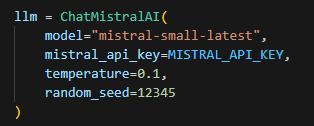
\includegraphics[width=.4\textwidth]{imagenes/0100_eval_gen_1.png}
			\caption{Configuración LLM de generación del conjunto de preguntas}		
			\label{fig:0100_eval_gen_1}
		\end{figure} 
		
		\noindent El siguiente paso en la generación del conjunto de preguntas es facilitar al modelo de lenguaje las instrucciones necesarias mediante un \textit{prompt} para generar el conjunto de preguntas. 
		
		\noindent Fijándose en la figura \ref{fig:0101_eval_gen_2}, el prompt hace especial hincapié en la necesidad del usuario de generar una única pregunta con su respuesta, siempre estando relacionado con la DANA y dado un determinado contexto. La pregunta debe mantener un formato muy específico y la salida debe presentarse separado por comas (para su posterior procesado en formato csv).
		
		\noindent El contexto aportado al final del prompt se refiere al contenido en texto de cada página de cada documento presente en la fuente de conocimiento, por lo que es necesario ejecutar el prompt varias veces en bucle. El número de ficheros que integraban dicha fuente en el momento de la generación de este conjunto de preguntas y respuestas era de alrededor de 80 con un total de más de 560 páginas.
		
		\begin{figure}[H]
			\centering
			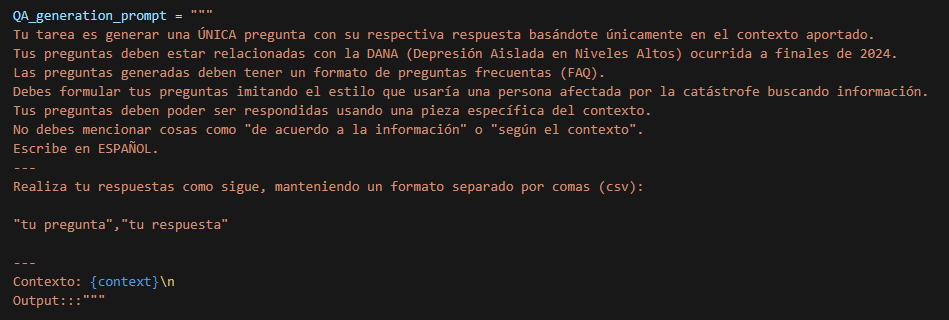
\includegraphics[width=1\textwidth]{imagenes/0101_eval_gen_2.png}
			\caption{Prompt usado en la generación del conjunto de preguntas}		
			\label{fig:0101_eval_gen_2}
		\end{figure} 
		
		\noindent Para añadir los documentos hemos vuelto a usar la clase \textit{PyPDFDirectoryLoader}, pasando como argumento la carpeta donde hemos descargado con anterioridad los ficheros de nuestra fuente de conocimiento. La figura \ref{fig:0103_eval_gen4} muestra este proceso y el de configuración inicial de la cadena \textit{chain}, siendo similar a lo mostrado con anterioridad en otros apartados.
		
		\begin{figure}[H]
			\centering
			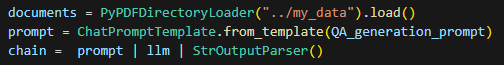
\includegraphics[width=0.6\textwidth]{imagenes/0103_eval_gen4.png}
			\caption{Carga de datos y preparación del modelo de lenguaje}		
			\label{fig:0103_eval_gen4}
		\end{figure} 
		
		\noindent El bucle antes mencionado, en el cual se deben generar todas las preguntas se puede apreciar en la figura \ref{fig:0102_eval_gen_3}. En dicha figura, se crea un fichero para albergar el conjunto entero de preguntas-respuestas, donde cada línea del fichero contendrá:
		
		\begin{itemize}
			\item \textbf{Pregunta:} La pregunta generada por el modelo de lenguaje.
			\item \textbf{Respuesta:} La respuesta a la pregunta generada por el modelo de lenguaje.
			\item \textbf{Contexto:} El contexto del cual se ha generado la pregunta.
			\item \textbf{Recurso:} El fichero del cual se ha conseguido el contexto.
		\end{itemize}
		
		\begin{figure}[H]
			\centering
			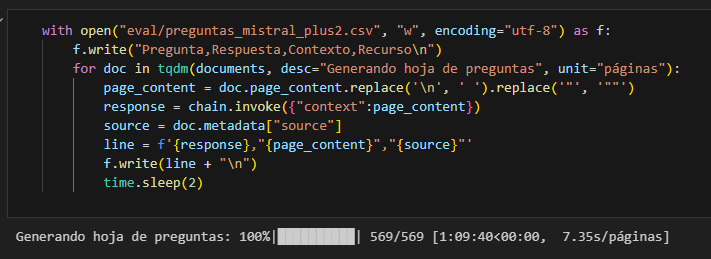
\includegraphics[width=0.8\textwidth]{imagenes/0102_eval_gen_3.png}
			\caption{Bucle para la generación del conjunto de preguntas}		
			\label{fig:0102_eval_gen_3}
		\end{figure} 
		
		\noindent La generación de este conjunto de preguntas ha tenido una duración en tiempo de una hora y diez minutos aproximadamente. La inclusión en el bucle de la parada (\textit{time.sleep(2)}) de dos segundos fue necesario para evitar el error por sobrecarga  del modelo (recordemos que es un modelo externo ofrecido de forma gratuita por \textit{Mistral AI}). Sin esta parada, la duración habría sido de alrededor de unos cincuenta minutos.
		
		\noindent El resultado final de la ejecución esta disponible en el recurso \cite{0042_pregu} de la bibliografía. El número final de preguntas se redujo a 300 debido a que existía bastante repetición entre las preguntas generadas. Una muestra de las quince primeras líneas de este fichero pueden observarse en la siguiente figura.
		
		\begin{figure}[H]
			\centering
			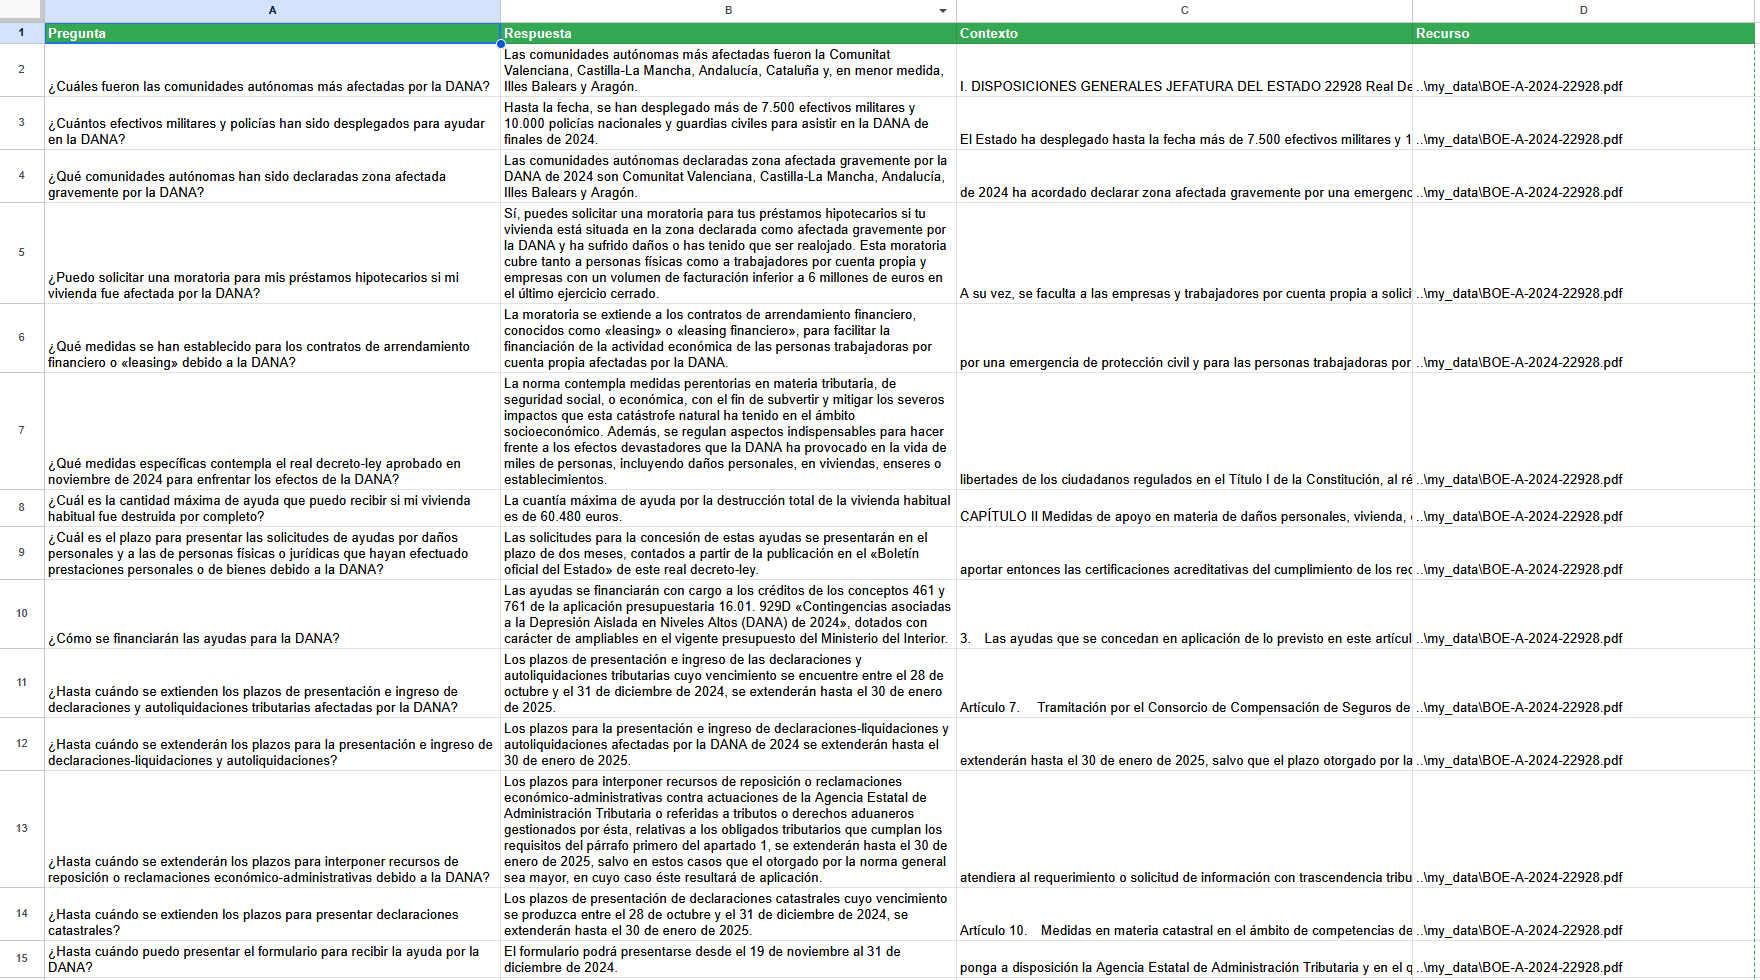
\includegraphics[width=1\textwidth]{imagenes/0103_eval_gen_4.png}
			\caption{Muestra del conjunto de preguntas \cite{0042_pregu}}		
			\label{fig:0103_eval_gen_4}
		\end{figure} 
		
		\noindent \textbf{Nota:} El fichero de generación de preguntas esta disponible en la raíz del proyecto \cite{0045_repo}, bajo el nombre \textbf{qa\_generator.ipynb} (formato Jupyter Notebook).
		
	\section{Configuración de las alternativas de evaluación}
	
		En este apartado veremos la parte que precede al segundo objetivo de este Trabajo de Fin de Máster, donde mostraremos la configuración de las opciones utilizadas para las pruebas del sistema RAG. Empezaremos hablando de los modelos usados para dichas pruebas, los cuales se encargarán tanto de generar las respuestas como de evaluarlas.
		
		\noindent \textbf{Nota:} El código de las siguientes figuras se puede encontrar en el fichero \textbf{rag\_eval.ipynb} del repositorio \cite{0045_repo}.
				
		\subsection{Modelos evaluadores y configuración inicial}
		
			Como ya hemos comentado en la última sección del capítulo \ref{2_metods_eva}, se harán estas pruebas en tres modelos: el modelo gratuito y local \textit{llama3.2}, el modelo gratuito pero externo \textit{mistral-small} y el modelo externo y de pago \textit{gpt-4.1}. La siguiente figura muestra tres imágenes de la configuración de cada uno de estos modelos usando \textit{LangChain}. Como es común para los modelos externos, debemos proporcionar su clave API para poder usarlos.
		
			\begin{figure}[H]
				\centering
				\begin{subfigure}{.32\textwidth}
					\centering
					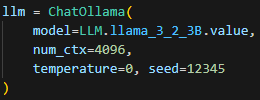
\includegraphics[width=1\textwidth]{imagenes/0106_eval_result3.png}
					\caption{Llama 3.2}
				\end{subfigure}   
				\begin{subfigure}{.32\textwidth}
					\centering
					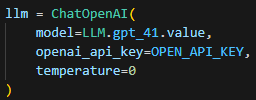
\includegraphics[width=1\textwidth]{imagenes/0105_eval_result2.png}
					\caption{GPT-4.1}
				\end{subfigure}        
				\begin{subfigure}{.32\textwidth}
					\centering
					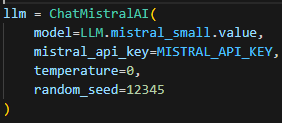
\includegraphics[width=1\textwidth]{imagenes/0104_eval_result1.png}
					\caption{Mistral Small 3.2}
				\end{subfigure}               
				\caption{Configuración de los modelos de lenguaje de pruebas}
				\label{fig:0106_eval_llms}
			\end{figure}  
			
			\noindent La variable \textit{model} común para todas las configuraciones de la figura anterior, contiene elementos de la clase \textit{LLM}. Estos elementos se corresponden con los nombres reales de los modelos que son usados para su acceso en la API y ya han sido mostrados en la figura \ref{fig:0082_llms}.
			
			\noindent El siguiente paso es configurar las demás variables de pruebas, la siguiente figura muestra alguna de ellas. En la primera línea podemos observar las estrategias de búsqueda que se probarán como mencionábamos en uno de los apartados de la sección \ref{2_metods_eva}. También observamos en la figura un \textit{prompt} que usaremos para medir la influencia en los resultados de un cambio en las instrucciones, en este caso más simples.
			
			\begin{figure}[H]
				\centering
				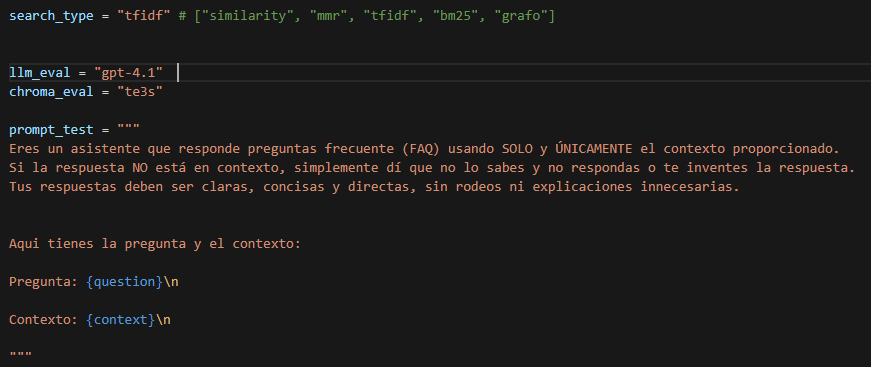
\includegraphics[width=.9\textwidth]{imagenes/0107_eval_result4.png}
				\caption{Variables de pruebas}		
				\label{fig:0107_eval_result4}
			\end{figure} 
			
			\noindent Las pruebas las realizaremos con dos \textit{chatbots}, la figura \ref{fig:0109_eval_result6} muestra la configuración de ambos. Los dos son exactamente iguales siendo el único cambio, el \textit{reranker} usado en el segundo de ellos (parte b). El caso de esta figura muestra una configuración de pruebas para modelos de \textit{OpenAI}, como se puede observar tanto por el modelo de lenguaje usado (\textit{gpt-4.1}) como por el de embedding (\textit{text-embedding-3-small}).
			
			\noindent Los modelos de embedding que probaremos están incluidos en la clase \textit{EMBEDDING} (ya mostrada en la figura \ref{fig:0081_chatbot}). El objetivo de la prueba de distintos modelos de embedding es dilucidar cual proporciona mejores resultados en la recuperación en conjunto con la generación de los modelos de lenguaje.
			
			\noindent \textbf{Nota:} Las clases \textit{LLM} y \textit{EMBEDDING} se encuentran en la carpeta \textit{classes} del repositorio \cite{0045_repo}.		 
			
			\begin{figure}[H]
				\centering
				\begin{subfigure}{.49\textwidth}
					\centering
					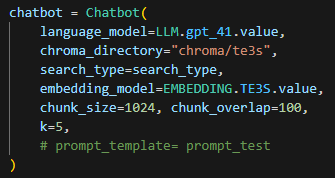
\includegraphics[width=1\textwidth]{imagenes/0108_eval_result5.png}
					\caption{Normal}
				\end{subfigure}   
				\begin{subfigure}{.49\textwidth}
					\centering
					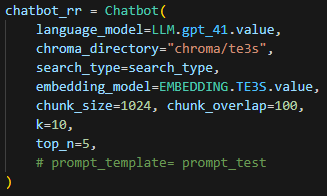
\includegraphics[width=1\textwidth]{imagenes/0109_eval_result6.png}
					\caption{Con reranker}
				\end{subfigure} 			
				\caption{Configuración de los chatbots de pruebas}
				\label{fig:0109_eval_result6}       
			\end{figure} 	
			
		\subsection{Agentes críticos}		
		
			Los agentes críticos son los encargados de realizar una evaluación de las respuestas generadas por los modelos de lenguaje. Las siguientes figuras muestran los \textit{prompts} con las instrucciones de los cuatro agentes críticos seleccionados para nuestras evaluaciones, y que están definidos en la sección \ref{2_metods_eva}.				
			
			\noindent El primero de ellos es el \textit{accuracy} (figura \ref{fig:0110_eval_result_agent1}), que es el encargado de evaluar la precisión de la respuesta generada por el modelo comparándola con la respuesta original. La figura muestra el \textit{prompt} con las instrucciones necesarias para que el modelo haga de evaluador comparando dos argumentos, e incluso, añadimos los criterios que tiene que seguir para asignar una nota.
			
			\noindent Todos los agentes evalúan de cero a cinco, siendo cero la peor nota y cinco la mejor.
			
			\begin{figure}[H]
				\centering
				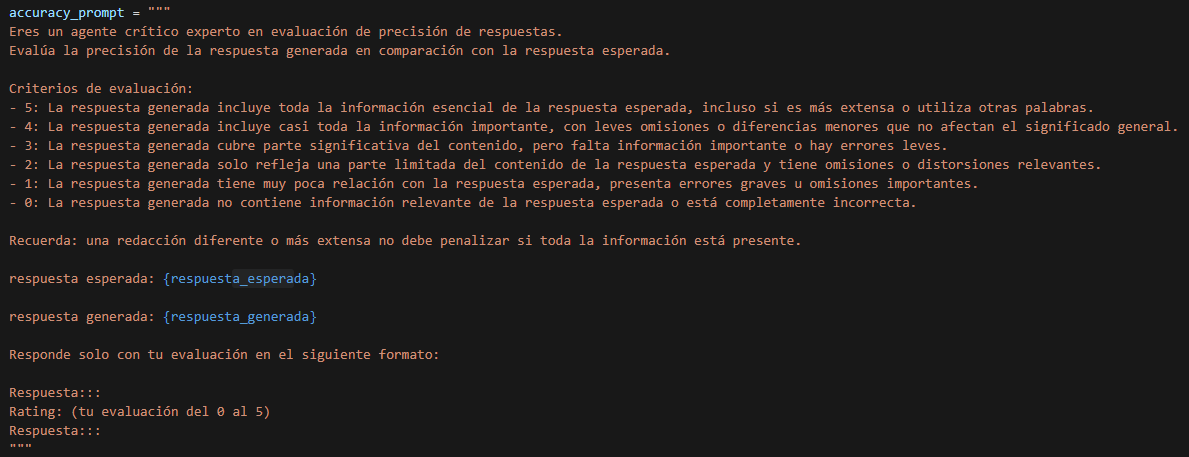
\includegraphics[width=1\textwidth]{imagenes/0110_eval_result_agent1.png}
				\caption{Agente crítico del accuracy}		
				\label{fig:0110_eval_result_agent1}
			\end{figure} 		
			
			\noindent El siguiente agente mide el \textit{faithfulness} (figura \ref{fig:0111_eval_result_agent2}). Esta medida evalúa el grado en que una respuesta esta basada en la información contenida en los documentos recuperados, por eso recibe estos dos argumentos. Gracias a esta medición obtenemos la fidelidad de la respuesta con los documentos de nuestra base de conocimiento.
			
			\begin{figure}[H]
				\centering
				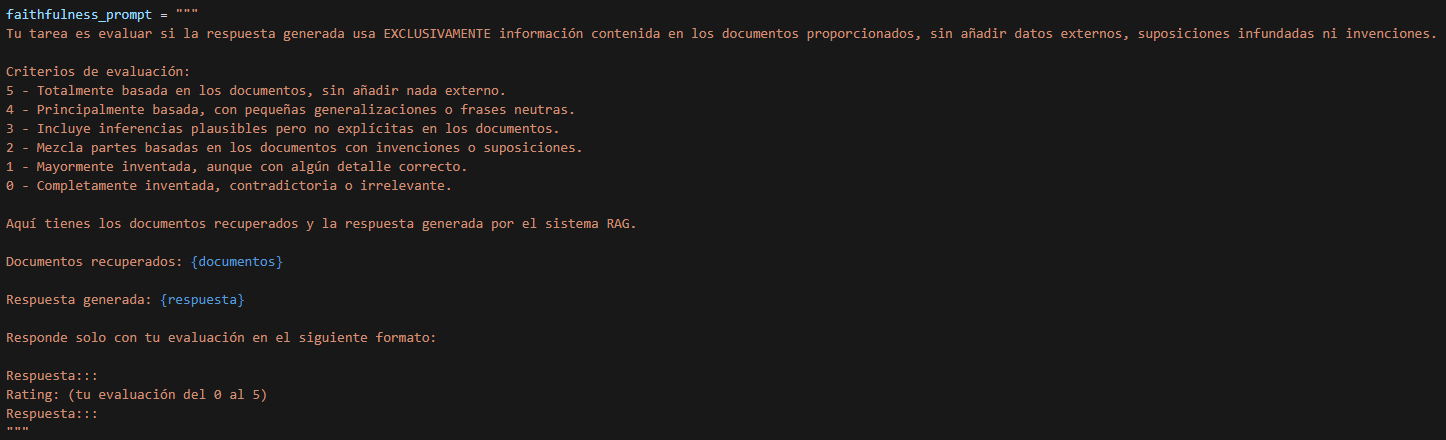
\includegraphics[width=1\textwidth]{imagenes/0111_eval_result_agent2.png}
				\caption{Agente crítico del faithfulness}		
				\label{fig:0111_eval_result_agent2}
			\end{figure} 	
			
			\noindent El \textit{groundedness} es una medida similar a la anterior (figura \ref{fig:0112_eval_result_agent3}), esta valora el uso de las evidencias aportadas por los documentos recuperados en la respuesta generada por el modelo. Es importante para mostrar lo bien (o mal) que usan la información disponible en los documentos recuperados a la hora de generar la respuesta.
			
			\begin{figure}[H]
				\centering
				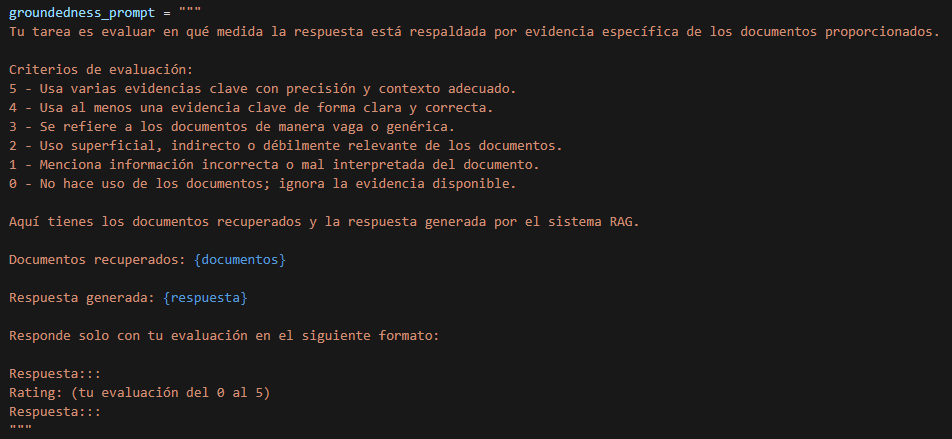
\includegraphics[width=1\textwidth]{imagenes/0112_eval_result_agent3.png}
				\caption{Agente crítico del groundedness}		
				\label{fig:0112_eval_result_agent3}
			\end{figure} 	
			
			\noindent El último agente se encarga de la relevancia (\textit{relevance}, figura \ref{fig:0113_eval_result_agent4}). La relevancia considera lo buenos que son los documentos recuperados para responder a la pregunta hecha y si se puede responder a ella de forma correcta, por eso recibe esos tres argumentos: pregunta, respuesta esperada y contexto (los documentos recuperados). Con esta medida podemos hacernos una idea de lo bien que funciona el modelo de recuperación de información (modelo de embedding) a la hora de responder preguntas, aportando documentos de calidad.
			
			\begin{figure}[H]
				\centering
				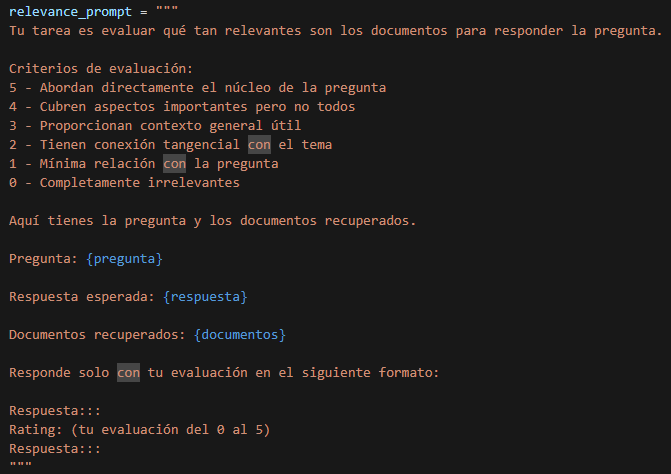
\includegraphics[width=.8\textwidth]{imagenes/0113_eval_result_agent4.png}
				\caption{Agente crítico de la relevancia}		
				\label{fig:0113_eval_result_agent4}
			\end{figure} 
			
		\subsection{Generación de evaluaciones}
		\label{sec:4_gen_evas}
		
			En este apartado abordaremos los pasos que hemos seguido para generar las evaluaciones de nuestro sistema RAG. Tal como sucedió en el apartado en el que generamos las preguntas de test (sección \ref{sec:4_gen_dataset}), necesitamos ejecutar un bucle en el que sean lanzadas todas las evaluaciones para cada pregunta. Esto incluye los siguientes pasos:
			
			\begin{enumerate}
				\item Generar la respuesta normal.
				\item Lanzar las evaluaciones a las respuestas normales.
				\item Generar la respuesta con reranking.
				\item Lanzar las evaluaciones a las respuestas con reranking.
				\item Guardar ambos resultados en formato csv.
			\end{enumerate}
			
			\noindent Usaremos como dataset de pruebas el conjunto de preguntas generado en la sección anterior. En la figura \ref{fig:0113_loadata} cargamos dicho conjunto en una variable ayudándonos de la clase \textit{pandas}, que permite una fácil lectura de ficheros csv. 
			
			\begin{figure}[H]
				\centering
				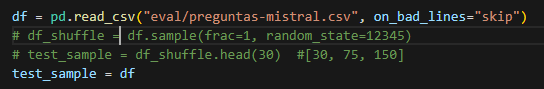
\includegraphics[width=.6\textwidth]{imagenes/0113_loadata.png}
				\caption{Carga de dataset de preguntas}		
				\label{fig:0113_loadata}
			\end{figure} 
			
			\noindent Antes de empezar el bucle de evaluaciones, necesitamos crear las variables que guardarán los resultados. La siguiente figura define dos variables para este propósito: \textit{eval\_rag} para las evaluaciones normales y \textit{eval\_rag\_rr} para las evaluaciones con \textit{reranking}. También se observa un \textit{array} de columnas, que será usado más tarde a la hora de guardar los resultados en ficheros.
		
			\begin{figure}[H]
				\centering
				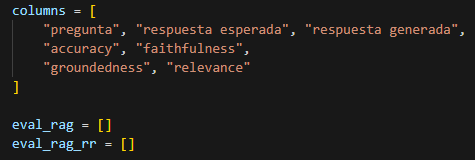
\includegraphics[width=.6\textwidth]{imagenes/0113_eval_result_test1.png}
				\caption{Columnas para el fichero de la evaluación y variables que contendrán los resultados de las evaluaciones}		
				\label{fig:0113_eval_result_test1}
			\end{figure} 
			
			\noindent Las funciones vistas en la figura \ref{fig:0115_eval_result_test2} son usadas dentro del bucle de preguntas para obtener la respuesta generada por el modelo de lenguaje y el contexto recuperado por el modelo de embedding. La primera, \textit{get\_response}, es usada para obtener los datos del modelo normal; y la segunda, obtiene los del modelo con \textit{reranking}. Ambas siguen una estructura similar pero muy simplificada de las usadas en la interfaz del \textit{chatbot}.
			
			\begin{figure}[H]
				\centering
				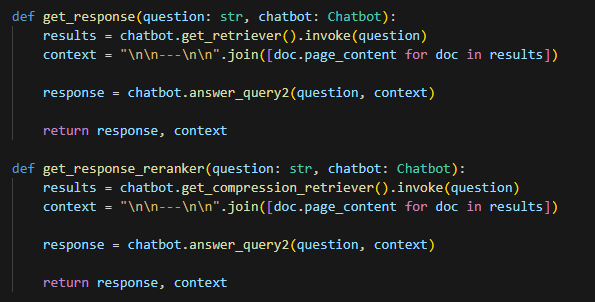
\includegraphics[width=.6\textwidth]{imagenes/0114_get_response.png}
				\caption{Función \textit{get\_response} y \textit{get\_response\_rr}, ambas usadas para generar respuestas en las pruebas}		
				\label{fig:0114_get_response}
			\end{figure} 
			
			\noindent El primer fragmento del bucle se puede apreciar en la siguiente figura. La imagen muestra el proceso que se sigue para cada pregunta, extrayendo y guardando los valores \textit{pregunta}, \textit{respuesta} y \textit{contexto} (este último no es usado). También genera una respuesta para cada pregunta y obtiene los documentos usados para construir la respuesta, ya que son necesarios para algunas evaluaciones de los agentes, que son formateados a continuación.			
			
			\begin{figure}[H]
				\centering
				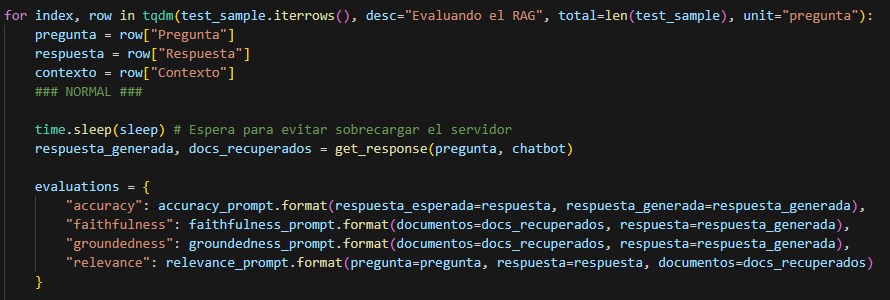
\includegraphics[width=.9\textwidth]{imagenes/0115_eval_result_test2.png}
				\caption{Fragmento 1 del bucle de evaluación de preguntas: se guardan datos del dataset de preguntas, se obtienen la respuesta generada y el contexto, y se formatean los agentes críticos}		
				\label{fig:0115_eval_result_test2}
			\end{figure} 
			
			\noindent El proceso para generar las respuestas y evaluaciones del modelo con \textit{reranking} es exactamente igual, en el que son usadas las mismas variables pero usando la terminación \textit{\_rr}. Por ejemplo, las evaluaciones de los agentes en la figura \ref{fig:0115_eval_result_test2} son guardadas en la variable \textit{evaluations}, así pues, en las del modelo con \textit{reranking} la variable se denomina \textit{evaluations\_rr}.
			
			\noindent Siguiendo con el proceso de generación de evaluaciones, queda lanzar los agentes. El proceso se puede observar en la figura \ref{fig:0116_eval_result_test3}. La imagen comienza creando una variable \textit{eval\_row} que contiene en principio la pregunta, respuesta original y respuesta generada, para en el siguiente bucle ir asignando y guardando uno a uno los resultados de las evaluaciones de los agentes. El bucle termina almacenando la variable \textit{eval\_row} en los resultados finales.
			
			\noindent Tal como ocurrió antes, el proceso de evaluación de los modelos con \textit{reranking} es exactemente igual, y las variables donde se almacenan sus resultados tienen la terminación \textit{\_rr}.
			
			\begin{figure}[H]
				\centering
				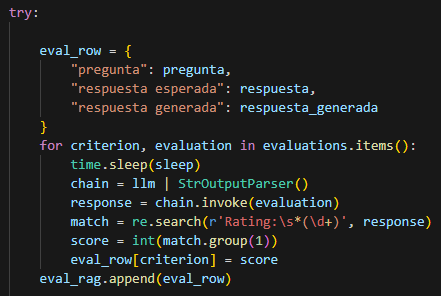
\includegraphics[width=.5\textwidth]{imagenes/0116_eval_result_test3.png}
				\caption{Fragmento 2 del bucle de evaluación de preguntas. Se van generando una a una las evaluaciones de los agentes}		
				\label{fig:0116_eval_result_test3}
			\end{figure} 
			
			\noindent Los resultados finales de ambos \textit{chatbots} son guardados individualmente y son impresos en formato csv, tal y como se indica en la siguiente figura. Hemos usado las variables de la figura \ref{fig:0107_eval_result4} para diferenciar las evaluaciones.
			
			\begin{figure}[H]
				\centering
				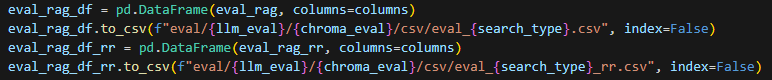
\includegraphics[width=.9\textwidth]{imagenes/0117_eval_result_save.png}
				\caption{Impresión de los resultados de los modelos en formato csv}		
				\label{fig:0117_eval_result_save}
			\end{figure} 
			
			\noindent Al realizar las evaluaciones, obtendremos varios ficheros con los resultados de cada una de ellas. Una muestra de lo que puede ocurrir se observa en la figura siguiente. Donde hemos realizado todas las evaluaciones disponibles para el conjunto \textit{GPT-4.1} y \textit{text-embedding-3-small}, resultando en diez ficheros.
			
			\begin{figure}[H]
				\centering
				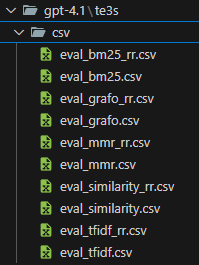
\includegraphics[width=.3\textwidth]{imagenes/0118_eval_result_save2.png}
				\caption{Contenido de la carpeta de evaluaciones \textit{GPT-4.1} en \textit{text-embedding-3-small}}		
				\label{fig:0118_eval_result_save2}
			\end{figure} 
			
			\noindent Cada fichero contiene la misma estructura, en la figura \ref{fig:0119_muestra_tfifg_rr_gpt} podemos ver el contenido del fichero correspondiente a la evaluación de búsqueda TF-IDF, sobre el par \textit{GPT-4.1}/\textit{text-embedding-3-small}. En este fragmento se puede apreciar tres preguntas con sus respectivas respuestas originales y generadas, y tambien, los resultados numéricos aportados por los agentes críticos.
			
			\begin{figure}[H]
				\centering
				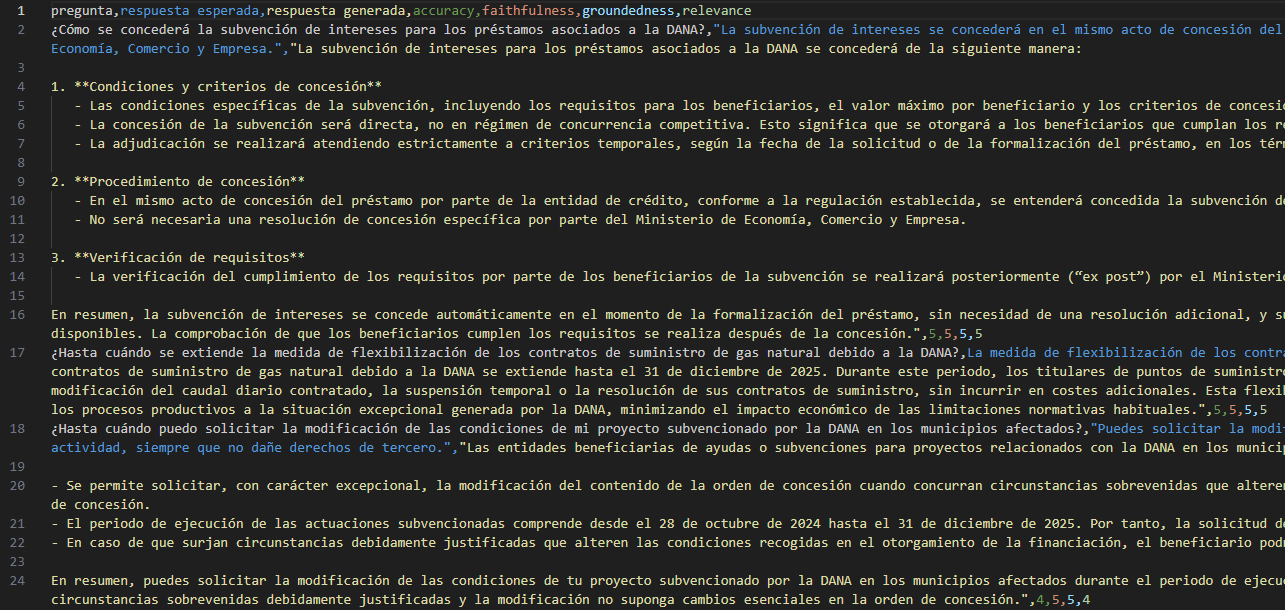
\includegraphics[width=1\textwidth]{imagenes/0119_muestra_tfifg_rr_gpt.png}
				\caption{Muestra del fichero de evaluaciones correspondiente al modelo de lenguaje \textit{GPT-4.1} y modelo de embedding \textit{text-embedding-3-small}, con la estrategia de búsqueda TF-IDF}		
				\label{fig:0119_muestra_tfifg_rr_gpt}
			\end{figure} 
			
			\noindent Una vez realizadas todas las pruebas que creamos oportunas, podemos generar fácilmente gráficas o tablas con los resultados de todas estas evaluaciones. La sección \ref{sec:4_results} tratará este tema más en profundidad.
    
    \section{Casos de uso de la aplicación}
    
    	En esta sección veremos los ejemplos de uso de la aplicación que hemos desarrollado. Algunos ya ha sido mostrados en el capítulo anterior, donde explicábamos los pasos seguidos en el diseño e implementación de la interfaz, apoyándonos con ejemplos de esta y código. 
    	
    	\noindent Los casos de uso que hemos elegido, representan el funcionamiento básico que obtendrá un usuario al interactuar con la interfaz web. Estos serán representados en una tabla informativa que mostrará: el nombre del caso de uso, los actores que interactúan en él, y las pre-condiciones y post-condiciones de dicho caso de uso. La plantilla usada se puede ver a continuación.
    	
    	\begin{table}[H]
    		\small
    		\centering
    		\begin{tblr}{
    				colspec = {p{3cm} p{9.5cm} p{1cm}},
    				column{1} = {CU1,fg=white},
    				column{3} = {CU2},
    				hlines,
    				vlines,
    			}
    			\textbf{Casos de uso} & << Nombre del CU >> &  << ID >>  \\
    			\textbf{Actores} & \SetCell[c=2]{wd=10.5cm,valign=t} << Listado de actores participantes en el CU >> & \\
    			\textbf{Pre-condiciones} & \SetCell[c=2]{wd=10.5cm,valign=t} << Condiciones que se tienen que dar para la realización del CU >> & \\
    			\textbf{Post-condiciones} &  \SetCell[c=2]{wd=10.5cm,valign=t} <<  Efectos tras la realización del CU >> &      
    		\end{tblr}
    		\caption{Plantilla usada en los casos de uso}
    		\label{tab:CU_template}
    	\end{table}
    	
    	El primer caso de uso \ref{tab:CU_01} representa el uso para el cual fue diseñada una interfaz, la interacción entre usuario y RAG mediante una consulta. 
    	
    	\begin{table}[H]
    		\small
    		\centering
    		\begin{tblr}{
    				colspec = {p{3cm} p{9.5cm} p{1cm}},
    				column{1} = {CU1,fg=white},
    				column{3} = {CU2},
    				hlines,
    				vlines,
    			}
    			\textbf{Casos de uso} & Pregunta: ``¿Cuál es la cantidad máxima que puedo recibir por daños en los electrodomésticos de mi vivienda actual debido a la DANA?" &  CU\_01  \\
    			\textbf{Actores} & \SetCell[c=2]{wd=10.5cm,valign=t} Usuario/Interfaz & \\
    			\textbf{Pre-condiciones} & \SetCell[c=2]{wd=10.5cm,valign=t} Sistema RAG completo: sistema de recuperación y generación de información & \\
    			\textbf{Post-condiciones} & \SetCell[c=2]{wd=10.5cm,valign=t} Respuesta informada con aportación de referencias &      
    		\end{tblr}
    		\caption{Caso de uso 01, consulta de usuario}
    		\label{tab:CU_01}
    	\end{table}
    	
    	\noindent La pre-condición de este caso de uso, implica que en la interacción entre usuario e interfaz deben estar todos los componentes del sistema RAG funcionando al 100\%, es decir: debe existir una base de conocimiento de la cual el modelo de recuperación de información extraerá la información/documentos pertinentes, y estos serán la base para generar una respuesta por el modelo de lenguaje que se use.
    	
    	\noindent Un ejemplo de empleo de este caso de uso fue mostrado en las ilustraciones \ref{fig:0095_interfaz4} y \ref{fig:0096_interfaz5} de esta memoria. 
    	
    	\noindent En cuanto a los dos siguientes casos de uso (\ref{tab:CU_02} y \ref{tab:CU_03}), representan algunos elementos de personalización en la respuesta. Podremos obtener respuestas usando un modelo de lenguaje distinto, o una recuperación distinta aplicando otra técnica de búsqueda.
    	
    	\noindent La interfaz muestra varias opciones como se pueden ver en las figuras \ref{fig:0122_CU_llms} y \ref{fig:0123_cu3}, y como ya se ha mencionado en secciones anteriores y en las pre-condiciones de los casos de uso, los modelos deben estar presentes en la máquina local o ser accesibles mediante API.
    	
    	\begin{table}[H]
    		\small
    		\centering
    		\begin{tblr}{
    				colspec = {p{3cm} p{9.5cm} p{1cm}},
    				column{1} = {CU1, fg=white},
    				column{3} = {CU2},
    				hlines,
    				vlines,
    			}
    			\textbf{Casos de uso} & Cambio de modelo de lenguaje en la consulta & CU\_02  \\
    			\textbf{Actores} & \SetCell[c=2]{wd=10.5cm,valign=t} Usuario/Interfaz & \\ 
    			\textbf{Pre-condiciones} & \SetCell[c=2]{wd=10.5cm,valign=t} Descarga previa en el caso de modelos locales, o acceso vía API a los modelos externos & \\ 
    			\textbf{Post-condiciones} & \SetCell[c=2]{wd=10.5cm,valign=t} Generación de respuesta usando el modelo elegido por el usuario &    
    		\end{tblr}
    		\caption{Caso de uso 02, cambio de LLM}
    		\label{tab:CU_02}
    	\end{table}
    	
    	\begin{figure}[H]
    		\centering
    		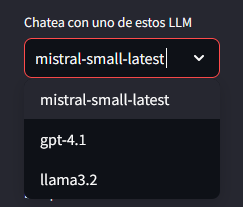
\includegraphics[width=.4\textwidth]{imagenes/0122_CU_llms.png}
    		\caption{Modelos de lenguaje disponibles en la interfaz web}		
    		\label{fig:0122_CU_llms}
    	\end{figure} 
    	
    	\begin{table}[H]
    		\small
    		\centering
    		\begin{tblr}{
    				colspec = {p{3cm} p{9.5cm} p{1cm}},
    				column{1} = {CU1,fg=white},
    				column{3} = {CU2},
    				hlines,
    				vlines,
    			}
    			\textbf{Casos de uso} & Cambio en la estrategia de búsqueda del modelo de recuperación &  CU\_03  \\
    			\textbf{Actores} & \SetCell[c=2]{wd=10.5cm,valign=t} Usuario/Interfaz & \\
    			\textbf{Pre-condiciones} & \SetCell[c=2]{wd=10.5cm,valign=t} Modelo de embedding disponible para realizar la recuperación & \\
    			\textbf{Post-condiciones} & \SetCell[c=2]{wd=10.5cm,valign=t} Recuperación de información usando la técnica elegida por el usuario &      
    		\end{tblr}
    		\caption{Caso de uso 03, cambio de estrategia de búsqueda}
    		\label{tab:CU_03}
    	\end{table}
    	
    	\begin{figure}[H]
    		\centering
    		\begin{subfigure}{.49\textwidth}
    			\centering
    			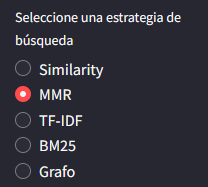
\includegraphics[width=.6\textwidth]{imagenes/0123_cu3_1.png}
    			\caption{Estrategia MMR}
    		\end{subfigure}   
    		\begin{subfigure}{.49\textwidth}
    			\centering
    			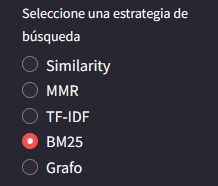
\includegraphics[width=.6\textwidth]{imagenes/0123_cu3_2.png}
    			\caption{Estrategia BM25}
    		\end{subfigure} 			
    		\caption{Ejemplos de cambio de estrategia de búsqueda desde la interfaz}
    		\label{fig:0123_cu3}       
    	\end{figure} 
    	  	
    	\noindent Los tres siguiente casos de uso se refieren tanto a la creación de la base de conocimiento del RAG, como a la actualización de esta. Es la base de un sistema RAG y lo que lo diferencia de un modelo de lenguaje genérico, el acceso a datos externos o privados.
    	
    	\noindent Nuestra interfaz cuenta con una página desde la que podemos cumplir el cometido de estos casos de uso: crear una base desde cero (\ref{tab:CU_04}), añadir nuevo conocimiento desde una carpeta (\ref{tab:CU_05}) o fichero (\ref{tab:CU_06}).
    	
    	\begin{table}[H]
    		\small
    		\centering
    		\begin{tblr}{
    				colspec = {p{3cm} p{9.5cm} p{1cm}},
    				column{1} = {CU1,fg=white},
    				column{3} = {CU2},
    				hlines,
    				vlines,
    			}
    			\textbf{Casos de uso} & Creación de base de conocimiento para el sistema RAG &  CU\_04  \\
    			\textbf{Actores} & \SetCell[c=2]{wd=10.5cm,valign=t} Usuario/Interfaz & \\
    			\textbf{Pre-condiciones} & \SetCell[c=2]{wd=10.5cm,valign=t} No existencia de base de datos vectorial, acceso a modelo de embedding local o vía API & \\
    			\textbf{Post-condiciones} & \SetCell[c=2]{wd=10.5cm,valign=t} Creación de base de datos vectorial con los documentos aportados &      
    		\end{tblr}
    		\caption{Caso de uso 04, creación de base vectorial}
    		\label{tab:CU_04}
    	\end{table}
    	
    	\begin{table}[H]
    		\small
    		\centering
    		\begin{tblr}{
    				colspec = {p{3cm} p{9.5cm} p{1cm}},
    				column{1} = {CU1,fg=white},
    				column{3} = {CU2},
    				hlines,
    				vlines,
    			}
    			\textbf{Casos de uso} & Actualizar de base de conocimiento desde carpeta &  CU\_05  \\
    			\textbf{Actores} & \SetCell[c=2]{wd=10.5cm,valign=t} Usuario/Interfaz & \\
    			\textbf{Pre-condiciones} & \SetCell[c=2]{wd=10.5cm,valign=t} Existencia de base de datos vectorial, acceso a modelo de embedding local o vía API y carpeta con documentos PDF & \\
    			\textbf{Post-condiciones} & \SetCell[c=2]{wd=10.5cm,valign=t} Nuevo conocimiento aportado a la base de datos vectorial desde la carpeta seleccionada &      
    		\end{tblr}
    		\caption{Caso de uso 05, actualización desde carpeta}
    		\label{tab:CU_05}
    	\end{table}   
    	
    	\begin{table}[H]
    		\small
    		\centering
    		\begin{tblr}{
    				colspec = {p{3cm} p{9.5cm} p{1cm}},
    				column{1} = {CU1,fg=white},
    				column{3} = {CU2},
    				hlines,
    				vlines,
    			}
    			\textbf{Casos de uso} & Actualizar de base de conocimiento desde fichero &  CU\_06  \\
    			\textbf{Actores} & \SetCell[c=2]{wd=10.5cm,valign=t} Usuario/Interfaz & \\
    			\textbf{Pre-condiciones} & \SetCell[c=2]{wd=10.5cm,valign=t} Existencia de base de datos vectorial, acceso a modelo de embedding local o vía API y fichero PDF  & \\
    			\textbf{Post-condiciones} & \SetCell[c=2]{wd=10.5cm,valign=t} Nuevo conocimiento aportado a la base de datos vectorial desde el fichero seleccionado &      
    		\end{tblr}
    		\caption{Caso de uso 06, actualización desde fichero}
    		\label{tab:CU_06}
    	\end{table} 
    	
    	\noindent Ejemplos de estos casos de uso ya fueron mostrados en el capítulo anterior, el contenido de la página visto en la figura \ref{fig:0075_update2}, y el resultado de la ejecución de los casos de uso \ref{tab:CU_05} y \ref{tab:CU_06} en las figuras \ref{fig:0078_waiting}, \ref{fig:0079_success1}, \ref{fig:0079_success2} y \ref{fig:0099_te3s-embed}.
    	
    \section{Resultados de las evaluaciones del RAG}
    \label{sec:4_results}
    
    	En esta sección presentaremos los resultados de las evaluaciones realizadas (disponibles en el anexo \cite{0044_results} de esta memoria) sobre el sistema RAG. En dichas evaluaciones se tomarán los resultados asignados por los cuatro agentes críticos definidos en el fichero de pruebas:
    	
    	\begin{itemize}
    		\item \textbf{Accuracy}: Evalúa la precisión de la respuesta generada en comparación a la respuesta esperada.
    		\item \textbf{Faithfulness}: Evalúa si la respuesta usa la información de los documentos recuperados.
    		\item \textbf{Groundness}: Evalúa la capacidad del modelo de apoyar sus respuestas en las evidencias de los documentos recuperados.
    		\item \textbf{Relevance}: Evalúa la relevancia de los documentos recuperados para responder a la pregunta.
    	\end{itemize}
    	
    	\noindent El conjunto de evaluación creado para la ocasión (ver sección \ref{sec:4_gen_dataset}) cuenta con un total de tres cientas preguntas con sus respectivas respuestas y referencias. Los agentes críticos realizarán sus evaluaciones pertinentes y guardarán los resultados en formato csv (como se indica en la sección \ref{sec:4_gen_evas}). Gracias al formato csv, podemos representar los resultados obtenidos por los agentes críticos en las diferentes configuraciones del sistema RAG de forma sencilla en forma de gráfica o de tabla.
    	
    	\noindent Antes de comenzar la sección de resultados, se han dispuesto las tablas \ref{tab:evo_preg1}, \ref{tab:evo_preg2} y \ref{tab:evo_preg3}. Estas muestran la respuesta generada por los LLMs usados a una misma pregunta, además de mostrar la respuesta original (base) y el accuracy asignado por el susodicho agente crítico. 
    	
    	\noindent Como se observa en todas las tablas, las respuestas generadas por los modelos de lenguaje son diferentes. El accuracy mostrado, obviamente, es afectado por la calidad de estas respuestas, diferenciando claramente al modelo Llama 3.2 (menos potente) de los otros dos. En las tablas \ref{tab:evo_preg2} y \ref{tab:evo_preg3} se observa claramente este factor: Llama 3.2 no puede o genera una respuesta incorrecta, lo que hace al agente crítico asignar la peor puntuación; mientras que los modelos de Mistral y OpenAI siempre generan respuestas buenas con puntuaciones altas (recordemos que las puntuaciones asignadas oscilan entre 1 para respuestas malas y 5 para respuestas buenas).
    	
    	\noindent \textbf{Nota:} Las muestras de las tablas se han extraído de las siguientes evaluaciones: modelo de embedding \textit{Jina} con tamaño de documento 1024 para \textit{Llama 3.2} y \textit{Mistral Small 3.2}, y modelo de embedding \textit{text-embedding3-small} con tamaño de documento 1024 para \textit{GPT-4.1}. La estrategia de búsqueda usada para todos ha sido \textit{similarity} con \textit{reranking}.
    	
    	\newpage
    	\begin{table}[H]
    		\small
    		\centering
    		\begin{tblr}{
    				colspec = {p{1.5cm} p{11cm} p{1.5cm}},
    				hlines,
    				vlines,
    			}
    			\textbf{Pregunta} & \SetCell[c=2]{wd=12cm,valign=t} ¿Cuánto dinero se ha movilizado en ayudas urgentes para hogares, empresas, autónomos e instituciones locales afectados por la DANA en la Comunitat Valenciana? & \\
    			\textbf{Respuesta base} & \SetCell[c=2]{wd=12cm,valign=t} 10.609 millones de euros & \\
    			\textbf{Modelo} & \textbf{Respuesta} & \textbf{Accuracy} \\
    			\textbf{Llama 3.2} & La respuesta es: Se han movilizado 10.609 millones de euros en ayudas urgentes para hogares, empresas, autónomos e instituciones locales afectados por la DANA en la Comunitat Valenciana.
    			
    			Esta información se encuentra en el contexto proporcionado, específicamente en el párrafo que describe las medidas adoptadas por el Gobierno para responder a los daños causados por la Depresión Aislada en Niveles Altos (DANA) en diferentes municipios de la Comunitat Valenciana. & 4 \\   	
    			 \textbf{Mistral Small 3.2} & El contexto proporcionado indica que, a través del **Real Decreto-ley 6/2024, de 5 de noviembre**, se han movilizado **10.609 millones de euros** en ayudas urgentes para hogares, empresas, autónomos e instituciones locales afectados por la DANA en la Comunitat Valenciana. Estas ayudas están destinadas a paliar daños personales, materiales en viviendas y enseres, así como en establecimientos industriales, mercantiles y de servicios.
    			 
    			 Además, el texto menciona que estas ayudas incluyen beneficios fiscales y de Seguridad Social, así como otras medidas complementarias. La movilización de estos fondos forma parte del **Plan de Respuesta Inmediata, de Reconstrucción y de Relanzamiento de la Comunitat Valenciana**, que busca abordar los efectos devastadores de la DANA en la región.
    			 
    			 No se especifica en el contexto si estos 10.609 millones de euros son exclusivos para la Comunitat Valenciana o si se distribuyen entre otras regiones afectadas. Sin embargo, el texto sí destaca que la DANA afectó a múltiples comunidades autónomas, incluyendo a la Comunitat Valenciana, donde se registraron daños en 75 términos municipales & 4 \\   
    			 \textbf{GPT-4.1} & Se han movilizado 10.609 millones de euros en ayudas urgentes para hogares, empresas, autónomos e instituciones locales afectados por la DANA en la Comunitat Valenciana. Estas ayudas forman parte de un primer conjunto de medidas implementadas el 5 de noviembre de 2024, destinadas a paliar daños personales, materiales en viviendas y enseres, así como en establecimientos industriales, mercantiles y de servicios. Además, se incluyen beneficios fiscales y de Seguridad Social, junto con otras medidas de protección social para los colectivos afectados en los municipios incluidos en el anexo del Real Decreto-ley 6/2024, de 5 de noviembre.
    			 
    			 Dentro de estas ayudas, se contemplan también subvenciones específicas, como:
    			 
    			 - 5.000.000 euros a la Plataforma del Tercer Sector para actuaciones en servicios sociales en los municipios afectados.
    			 - 700.000 euros al Consejo General de Trabajo Social para el refuerzo y despliegue del Grupo Estatal de Intervención en Emergencias Sociales (GEIES).
    			 
    			 Estas ayudas son compatibles con otras subvenciones, ayudas, ingresos o recursos que puedan recibir los beneficiarios. Además, se han previsto convocatorias específicas para entidades locales especialmente afectadas, y se han detallado importes concretos para municipios como València-Pedanías Sur, Vilamarxant, Yátova y Benicull de Xúquer, entre otros.
    			 
    			 En resumen, el total movilizado en ayudas urgentes asciende a 10.609 millones de euros, incluyendo tanto ayudas directas como subvenciones y otras medidas de apoyo económico y social. & 4 \\       			 		    			
    		\end{tblr}
    		\caption{Comparativa de respuestas a pregunta 1}
    		\label{tab:evo_preg1}
    	\end{table} 
    	
    	\begin{table}[H]
    		\small
    		\centering
    		\begin{tblr}{
    				colspec = {p{1.5cm} p{11cm} p{1.5cm}},
    				hlines,
    				vlines,
    			}
    			\textbf{Pregunta} & \SetCell[c=2]{wd=12cm,valign=t} ¿Dónde puedo adquirir los vehículos subvencionados por el PLAN REINICIA AUTO+? & \\
    			\textbf{Respuesta base} & \SetCell[c=2]{wd=12cm,valign=t} Los vehículos objeto de las subvenciones solo podrán adquirirse a través de los puntos de venta acreditados en el programa PLAN REINICIA AUTO+. & \\
    			\textbf{Modelo} & \textbf{Respuesta} & \textbf{Accuracy} \\
    			\textbf{Llama 3.2} & No puedo proporcionar una respuesta detallada a la pregunta. ¿Puedo ayudarte con algo más? & 1 \\   	
    			\textbf{Mistral Small 3.2} & Los vehículos subvencionados por el **PLAN REINICIA AUTO+** solo pueden adquirirse a través de los **puntos de venta acreditados** en dicho programa. Esta adquisición debe realizarse siguiendo el **procedimiento establecido en el artículo 9** de la convocatoria.
    			
    			Además, el ámbito geográfico de estas operaciones de compraventa abarca **todo el territorio nacional**, lo que significa que los puntos de venta acreditados pueden estar ubicados en cualquier parte de España.
    			
    			En resumen:
    			- **Lugar de adquisición**: Puntos de venta acreditados en el PLAN REINICIA AUTO+.
    			- **Procedimiento**: Según lo indicado en el artículo 9.
    			- **Ámbito geográfico**: Todo el territorio nacional. & 4 \\   
    			\textbf{GPT-4.1} & Los vehículos subvencionados por el PLAN REINICIA AUTO+ solo pueden adquirirse a través de los puntos de venta acreditados en el propio programa PLAN REINICIA AUTO+. No es posible comprarlos en cualquier concesionario, sino únicamente en aquellos que estén reconocidos y acreditados dentro del programa.
    			
    			El ámbito geográfico para la adquisición de estos vehículos abarca todo el territorio nacional, por lo que puedes acceder a los puntos de venta acreditados en cualquier parte de España.
    			
    			Para adquirir un vehículo subvencionado, debes seguir el procedimiento establecido en el artículo 9 del programa. Tanto los vehículos nuevos matriculados en España a partir del 30 de octubre de 2024, como los vehículos seminuevos que hayan sido titularidad de un concesionario y matriculados a su nombre después del 30 de octubre de 2021, pueden ser objeto de ayuda, siempre que la compra se realice en estos puntos de venta acreditados.
    			
    			En resumen:
    			
    			- Los vehículos subvencionados solo pueden adquirirse en puntos de venta acreditados en el PLAN REINICIA AUTO+.
    			- El ámbito de adquisición es todo el territorio nacional.
    			- Es necesario seguir el procedimiento específico del programa para la compra.
    			
    			No se proporciona en el contexto una lista concreta de los puntos de venta acreditados, pero estos deben estar identificados oficialmente dentro del programa PLAN REINICIA AUTO+. & 5 \\       			 		    			
    		\end{tblr}
    		\caption{Comparativa de respuestas a pregunta 2}
    		\label{tab:evo_preg2}
    	\end{table} 
    	
    	\begin{table}[H]
    		\small
    		\centering
    		\begin{tblr}{
    				colspec = {p{1.5cm} p{11cm} p{1.5cm}},
    				hlines,
    				vlines,
    			}
    			\textbf{Pregunta} & \SetCell[c=2]{wd=12cm,valign=t} ¿Qué entidad está a cargo del seguimiento de la calidad de las aguas continentales afectadas por la DANA en octubre de 2024 en la Confederación Hidrográfica del Júcar? & \\
    			\textbf{Respuesta base} & \SetCell[c=2]{wd=12cm,valign=t} La Presidencia de la Confederación Hidrográfica del Júcar es la entidad encargada del seguimiento de la calidad de las aguas continentales afectadas por la DANA en octubre de 2024. & \\
    			\textbf{Modelo} & \textbf{Respuesta} & \textbf{Accuracy} \\
    			\textbf{Llama 3.2} & La entidad a cargo del seguimiento de la calidad de las aguas continentales afectadas por la DANA en octubre de 2024 en la Confederación Hidrográfica del Júcar es el Ministerio para la Transición Ecológica y el Reto Demográfico. & 1 \\   	
    			\textbf{Mistral Small 3.2} & La entidad encargada del seguimiento de la calidad de las aguas continentales afectadas por la DANA en octubre de 2024 en la Confederación Hidrográfica del Júcar es la **Presidencia de la Confederación Hidrográfica del Júcar**. Esta responsabilidad se detalla en el anuncio de formalización de contratos publicado en el Boletín Oficial del Estado (BOE) el 13 de marzo de 2025, bajo el expediente **FP.CAC.002/2025**. El objeto del contrato es específicamente el **seguimiento de la calidad de las aguas continentales** para evaluar la afección causada por las avenidas de agua extraordinarias derivadas de los fuertes temporales provocados por la DANA en octubre de 2024.
    			
    			Además, se proporcionan los siguientes datos de contacto de la entidad:
    			- **Dirección**: Av. Blasco Ibañez 48, Valencia (46010).
    			- **Teléfono**: 963938816.
    			- **Fax**: 963938801.
    			- **Número de identificación fiscal**: Q4617001E.
    			
    			Esta información está respaldada por el anuncio oficial publicado en el BOE, que especifica que la Presidencia de la Confederación Hidrográfica del Júcar es la responsable de este seguimiento. & 5 \\   
    			\textbf{GPT-4.1} & La entidad a cargo del seguimiento de la calidad de las aguas continentales afectadas por la DANA en octubre de 2024 en el ámbito de la Confederación Hidrográfica del Júcar es la Presidencia de la Confederación Hidrográfica del Júcar. Esta entidad tiene como objeto la evaluación de la afección causada por las avenidas de agua extraordinarias derivadas de los fuertes temporales provocados por la DANA en dicho periodo.
    			
    			Los datos relevantes de la entidad responsable son:
    			
    			- Nombre: Presidencia de la Confederación Hidrográfica del Júcar
    			- Dirección: Av. Blasco Ibañez 48, Valencia, 46010, España
    			- Teléfono: 963938816
    			- Fax: 963938801
    			- Correo electrónico: Bzn\_Contratacion@chj.es
    			- Página web: http://www.chj.es/
    			
    			La actividad principal ejercida por esta autoridad estatal es la protección del medio ambiente, y el seguimiento de la calidad de las aguas continentales se realiza específicamente para evaluar los efectos de la DANA de octubre de 2024 en el ámbito de la Confederación Hidrográfica del Júcar. & 5 \\       			 		    			
    		\end{tblr}
    		\caption{Comparativa de respuestas a pregunta 3}
    		\label{tab:evo_preg3}
    	\end{table} 
    	
    	\subsection{Resultados de Mistral Small 3.2}
    	
    		El modelo \textit{Mistral Small 3.2}, es sobre el cual hemos realizado el mayor numero de observaciones. El carácter externo y gratuito de este modelo nos ha permitido ejecutar al menos una prueba con cada modelo de embedding disponible localmente en sus diferentes versiones (tamaño 512 y 1024 de documentos) y con distintos \textit{prompts}, en unos tiempos moderadamente bajos. 
    		
    		\noindent Cada prueba de modelo de embedding y estrategia de búsqueda tomaba alrededor de 3 horas de ejecución. Si hacemos cuentas del tiempo empleado solo en pruebas de este modelo de lenguaje, obtendríamos un total de 240 horas empleadas para generar los resultados sólo de esta sección (los resultados sin y con \textit{reranking} se obtienen en una misma prueba).
    		
    		\noindent En los siguientes apartados se muestran los resultados obtenidos en tablas y gráficas de las evaluaciones realizadas, junto con breves observaciones de ellos.
    	
    		\subsubsection{Resultados en bases de datos con tamaño de documentos 512}
    		
    			En las primeras pruebas hemos usado las bases de datos con menor tamaño (512). Los resultados pueden verse en la siguiente tabla, que esta ordenaba por el mejor \textit{accuracy} de cada modelo de embedding.
    	
    			\newpage
		    	\begin{table}[H]
		    		\centering
		    		\tiny
		    		\begin{tblr}{
		    				row{1} = {bg=white}, 
		    				row{2-11} = {bg=yellow!20}, 
		    				row{12-21} = {bg=green!20},    				
		    				row{22-31} = {bg=blue!20}, 
		    				row{32-41} = {bg=violet!20}, 
		    				hlines,
		    				vlines,
		    			}
		    			\textbf{Embedding} & \textbf{Estrategia} & \textbf{Accuracy} & \textbf{Faithfulness} & \textbf{Groundedness} & \textbf{Relevance} \\
		    			bge-m3 & tfidf\_rr & \SetCell{bg=yellow} \textbf{3.46} & 4.79 & \SetCell{bg=yellow} \textbf{4.71} & \SetCell{bg=yellow} \textbf{4.51} \\
		    			bge-m3 & tfidf & 3.36 & 4.78 & 4.59 & 4.34 \\
		    			bge-m3 & bm25\_rr & 3.3 & \SetCell{bg=yellow} \textbf{4.8} & 4.57 & 4.37 \\
		    			bge-m3 & grafo\_rr & 3.19 & 4.75 & 4.62 & 4.12 \\
		    			bge-m3 & similarity\_rr & 3.15 & 4.78 & 4.65 & 4.24 \\
		    			bge-m3 & bm25 & 3.14 & 4.73 & 4.41 & 4.15 \\
		    			bge-m3 & mmr\_rr & 3.13 & 4.79 & 4.64 & 4.24 \\
		    			bge-m3 & similarity & 3.1 & 4.75 & 4.57 & 4.14 \\
		    			bge-m3 & grafo & 3.03 & 4.76 & 4.5 & 4.1 \\
		    			bge-m3 & mmr & 2.91 & 4.79 & 4.45 & 4.07 \\
		    			jina & tfidf\_rr & \SetCell{bg=green}\textbf{3.52} & 4.77 & \SetCell{bg=green}\textbf{4.66} & \SetCell{bg=green}\textbf{4.5} \\
		    			jina & tfidf & 3.39 & 4.8 & 4.59 & 4.33 \\
		    			jina & bm25\_rr & 3.28 & 4.76 & 4.6 & 4.37 \\
		    			jina & mmr\_rr & 3.15 & 4.76 & 4.63 & 4.21 \\
		    			jina & bm25 & 3.14 & 4.67 & 4.39 & 4.15 \\
		    			jina & similarity\_rr & 3.13 & \SetCell{bg=green}\textbf{4.84} & \SetCell{bg=green}\textbf{4.66} & 4.32 \\
		    			jina & grafo\_rr & 3.03 & 4.79 & 4.58 & 3.97 \\
		    			jina & mmr & 3.02 & 4.79 & 4.48 & 4.14 \\
		    			jina & similarity & 2.94 & 4.78 & 4.59 & 4.1 \\
		    			jina & grafo & 2.92 & 4.77 & 4.45 & 3.85 \\
		    			nomic & tfidf\_rr & \SetCell{bg=blue!50}\textbf{3.5} & 4.8 & \SetCell{bg=blue!50}\textbf{4.68} & \SetCell{bg=blue!50}\textbf{4.49} \\
		    			nomic & tfidf & 3.39 & 4.77 & 4.52 & 4.28 \\
		    			nomic & bm25\_rr & 3.33 & 4.78 & 4.59 & 4.38 \\
		    			nomic & similarity\_rr & 3.28 & \SetCell{bg=blue!50}\textbf{4.81} & 4.59 & 4.33 \\
		    			nomic & mmr\_rr & 3.23 & 4.78 & 4.54 & 4.27 \\
		    			nomic & similarity & 3.17 & 4.76 & 4.52 & 4.14 \\
		    			nomic & bm25 & 3.11 & 4.75 & 4.35 & 4.12 \\
		    			nomic & grafo\_rr & 3.09 & 4.76 & 4.5 & 4.06 \\
		    			nomic & grafo & 3.01 & 4.77 & 4.39 & 3.97 \\
		    			nomic & mmr & 2.93 & 4.74 & 4.28 & 3.99 \\
		    			snowflake & tfidf\_rr & \SetCell{bg=violet!50}\textbf{3.51} & 4.78 & 4.67 & \SetCell{bg=violet!50}\textbf{4.5} \\
		    			snowflake & similarity\_rr & 3.49 & 4.82 & \SetCell{bg=violet!50}\textbf{4.74} & 4.49 \\
		    			snowflake & similarity & 3.44 & 4.8 & 4.66 & 4.38 \\
		    			snowflake & mmr\_rr & 3.43 & 4.82 & 4.69 & 4.5 \\
		    			snowflake & tfidf & 3.39 & 4.79 & 4.63 & 4.33 \\
		    			snowflake & bm25\_rr & 3.34 & 4.79 & 4.61 & 4.36 \\
		    			snowflake & grafo\_rr & 3.32 & 4.8 & 4.67 & 4.35 \\
		    			snowflake & grafo & 3.3 & 4.77 & 4.6 & 4.23 \\
		    			snowflake & mmr & 3.29 & \SetCell{bg=violet!50}\textbf{4.84} & 4.62 & 4.32 \\
		    			snowflake & bm25 & 3.15 & 4.74 & 4.38 & 4.14 \\
		    		\end{tblr}
		    		\caption{Resultados de Mistral Small 3.2 en embeddings con 512 de tamaño de documentos}
		    		\label{tab:result_mistral_512}
		    	\end{table}
		    	
		    	\noindent Los resultados obtenidos de las pruebas según la tabla anterior, muestran una clara superioridad de la estrategia de búsqueda \textit{TF-IDF} con \textit{reranking} sobre las demás al menos en el \textit{accuracy}, siendo \textit{JINA} el mejor modelo de embedding en este apartado. El modelo \textit{JINA} esta entrenado principalmente en español, por lo que es lógico que obtenga los mejores resultados.
		    	
		    	\noindent Los demás agentes representan lo bien que es utilizado el contexto en las respuestas o la relevancia de este a la hora de responder, y sus resultados son muy parecidos en las distintas estrategias y modelos. Salvando algunas excepciones, en general los resultados de estos últimos agentes son bastante altos, lo que indica que las respuestas están bien fundamentadas y el contexto recuperado es bueno.
		    	
		    	\noindent En cuanto al \textit{accuracy}, es un factor que debe mejorar. El mejor resultado, 3.52 sobre 5 no es muy alto, veremos si mejora en las siguientes pruebas.
		    	
		    	\noindent Como aporte final para este apartado, las siguientes cuatro gráficas muestran el contenido que puede verse en la tabla \ref{tab:result_mistral_512} de forma individual y separando los resultado sin y con \textit{reranking}. 
		    	
		    	\begin{figure}[H]
		    		\centering
		    		\begin{subfigure}{.49\textwidth}
		    			\centering
		    			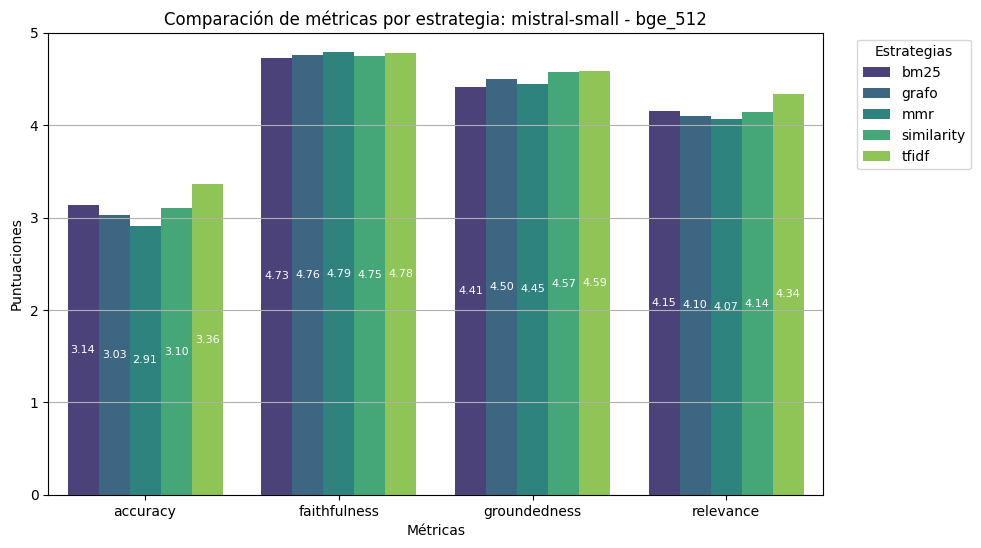
\includegraphics[width=1\textwidth]{imagenes/0124_bge_512.png}
		    			\caption{Sin reranking}
		    		\end{subfigure}   
		    		\begin{subfigure}{.49\textwidth}
		    			\centering
		    			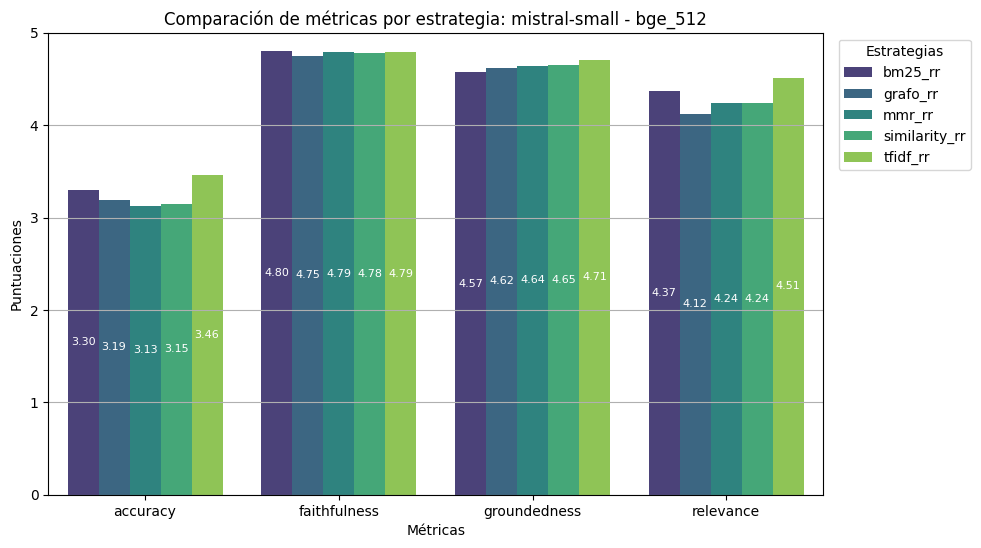
\includegraphics[width=1\textwidth]{imagenes/0124_bge_rr_512.png}
		    			\caption{Con reranking}
		    		\end{subfigure} 			
		    		\caption{Gráfica de rendimiento del modelo Mistral Small 3.2 usando el modelo de embedding BGE-M3 y tamaños de documento 512}
		    		\label{fig:0124_bge_512}       
		    	\end{figure} 
		    	
		    	\begin{figure}[H]
		    		\centering
		    		\begin{subfigure}{.49\textwidth}
		    			\centering
		    			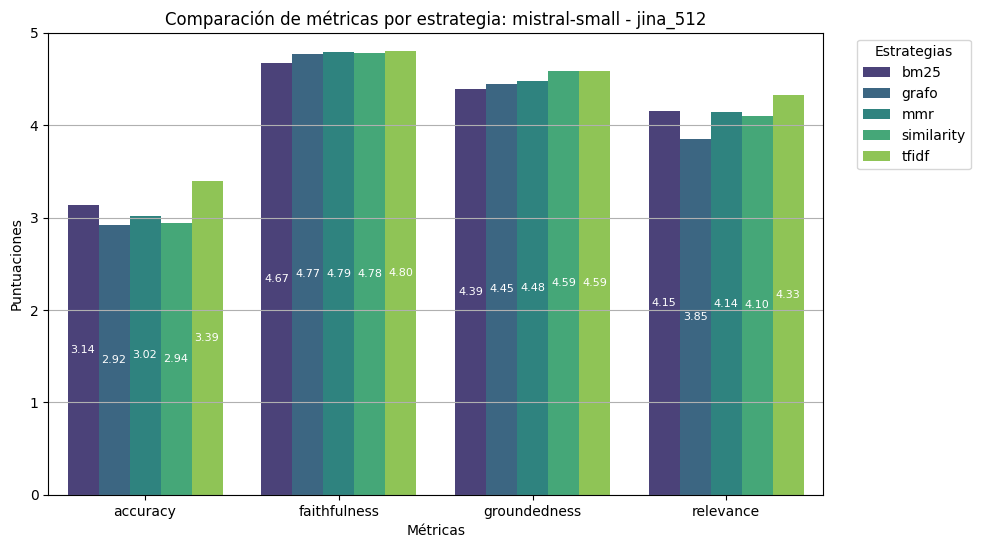
\includegraphics[width=1\textwidth]{imagenes/0125_jina_512.png}
		    			\caption{Sin reranking}
		    		\end{subfigure}   
		    		\begin{subfigure}{.49\textwidth}
		    			\centering
		    			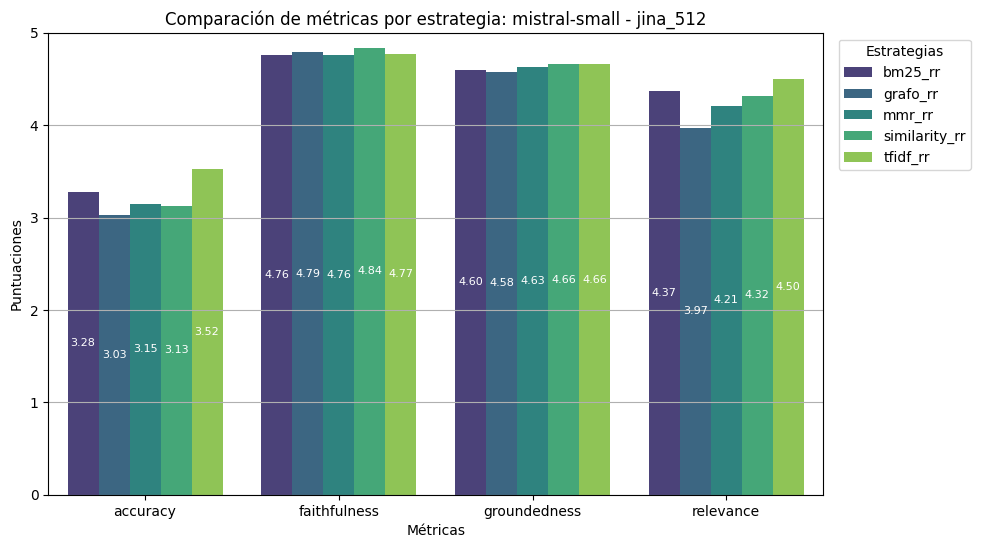
\includegraphics[width=1\textwidth]{imagenes/0125_jina_rr_512.png}
		    			\caption{Con reranking}
		    		\end{subfigure} 			
		    		\caption{Gráfica de rendimiento del modelo Mistral Small 3.2 usando el modelo de embedding JINA y tamaños de documento 512}
		    		\label{fig:0125_jina_512}       
		    	\end{figure} 
		    	
		    	\begin{figure}[H]
		    		\centering
		    		\begin{subfigure}{.49\textwidth}
		    			\centering
		    			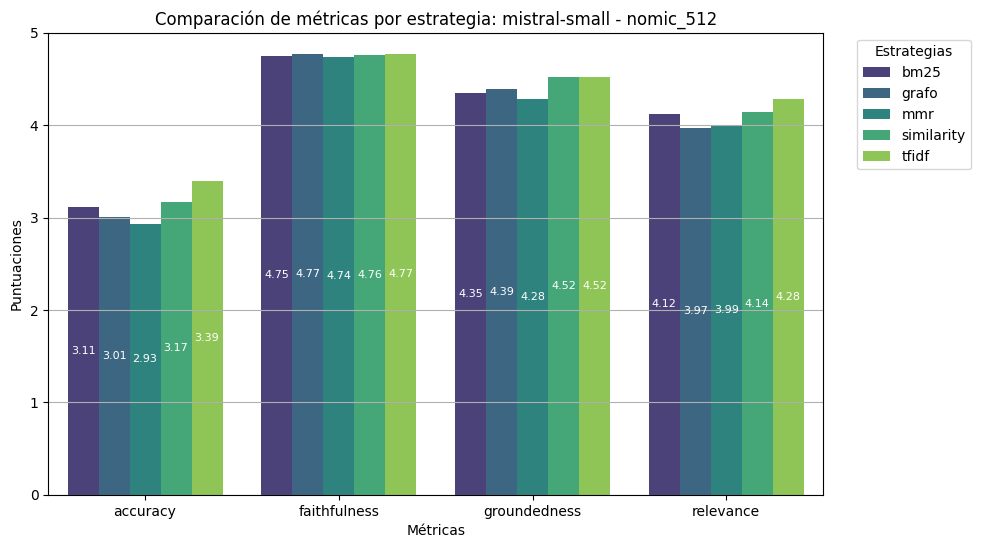
\includegraphics[width=1\textwidth]{imagenes/0126_nomic_512.png}
		    			\caption{Sin reranking}
		    		\end{subfigure}   
		    		\begin{subfigure}{.49\textwidth}
		    			\centering
		    			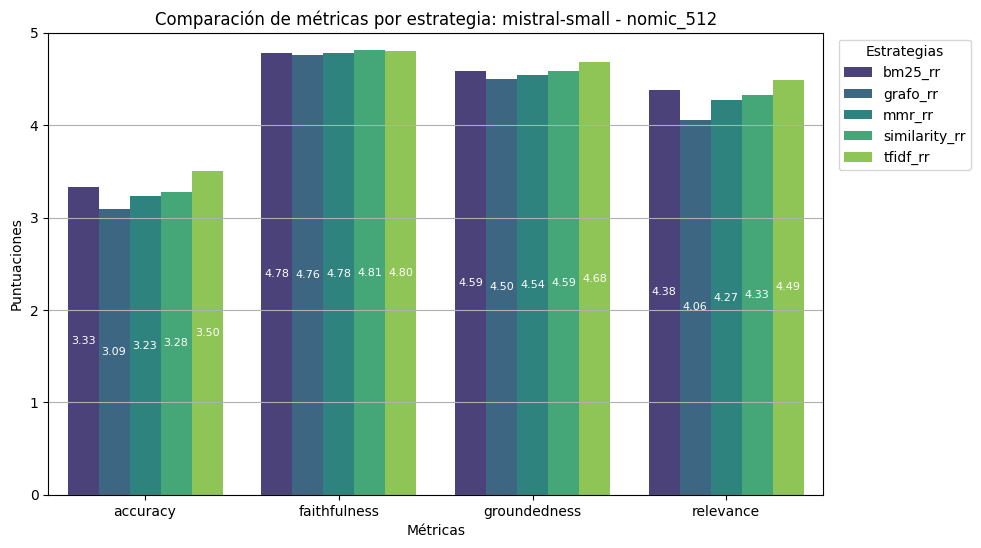
\includegraphics[width=1\textwidth]{imagenes/0126_nomic_rr_512.png}
		    			\caption{Con reranking}
		    		\end{subfigure} 			
		    		\caption{Gráfica de rendimiento del modelo Mistral Small 3.2 usando el modelo de embedding Nomic-Embed-Text y tamaños de documento 512}
		    		\label{fig:0126_nomic_512}       
		    	\end{figure} 
		    	
		    	\begin{figure}[H]
		    		\centering
		    		\begin{subfigure}{.49\textwidth}
		    			\centering
		    			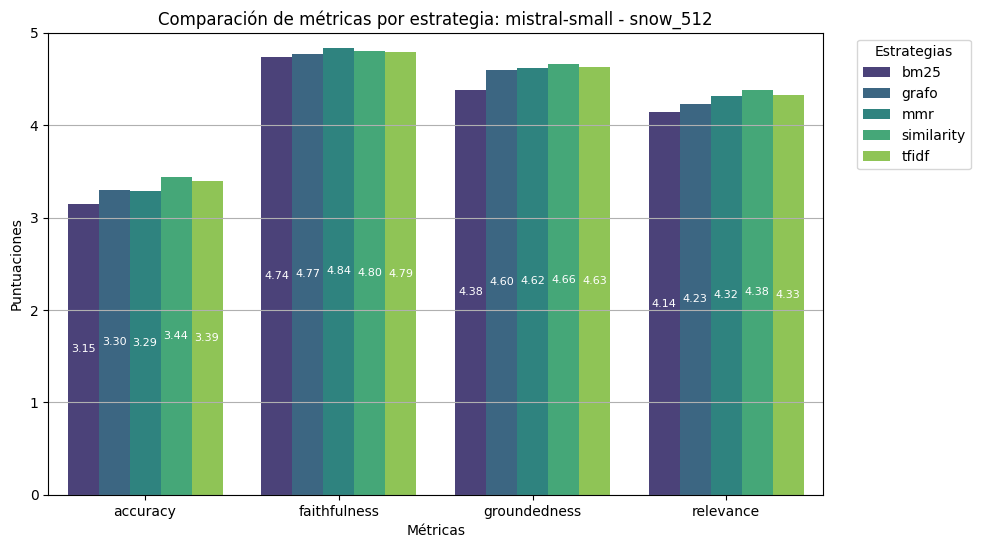
\includegraphics[width=1\textwidth]{imagenes/0127_snow_512.png}
		    			\caption{Sin reranking}
		    		\end{subfigure}   
		    		\begin{subfigure}{.49\textwidth}
		    			\centering
		    			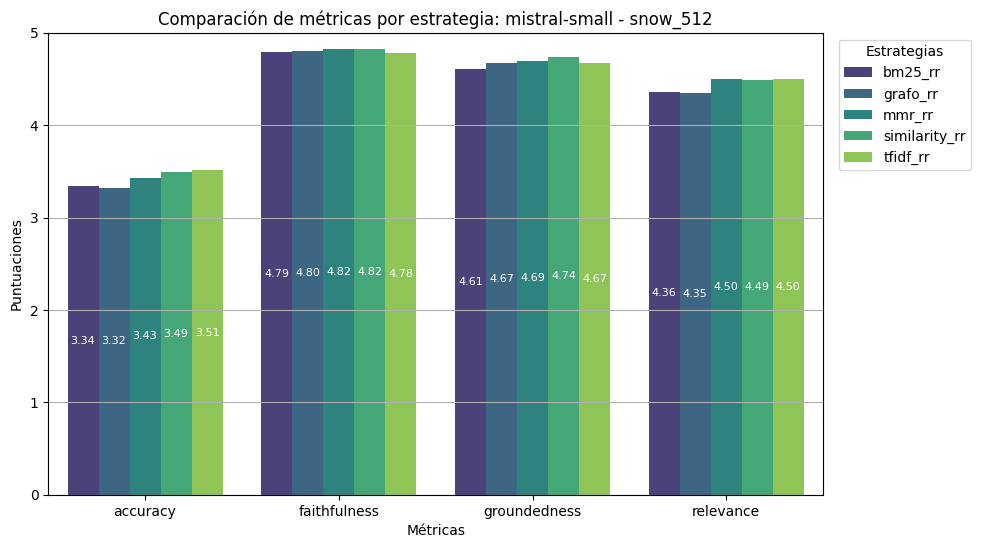
\includegraphics[width=1\textwidth]{imagenes/0127_snow_rr_512.png}
		    			\caption{Con reranking}
		    		\end{subfigure} 			
		    		\caption{Gráfica de rendimiento del modelo Mistral Small 3.2 usando el modelo de embedding Snowflakev2 y tamaños de documento 512}
		    		\label{fig:0127_snow_512}       
		    	\end{figure} 
		    

	    	\subsubsection{Resultados en bases de datos con tamaño de documentos 1024}
	    	
	    		En la segunda tanda de pruebas se usaron las bases de datos con mayor tamaño (1024). Los resultados pueden verse en la siguiente tabla, que esta ordenaba por el mejor \textit{accuracy} de cada modelo de embedding.
	    	
	    		\newpage
	    		\begin{table}[H]
	    			\centering
	    			\tiny
	    			\begin{tblr}{
	    					row{1} = {bg=white}, 
	    					row{2-11} = {bg=yellow!20}, 
	    					row{12-21} = {bg=green!20},    				
	    					row{22-31} = {bg=blue!20}, 
	    					row{32-41} = {bg=violet!20}, 
	    					hlines,
	    					vlines,
	    				}
	    				\textbf{Embedding} & \textbf{Estrategia} & \textbf{Accuracy} & \textbf{Faithfulness} & \textbf{Groundedness} & \textbf{Relevance} \\
	    				bge-m3 & tfidf\_rr & \SetCell{bg=yellow}\textbf{3.77} & 4.91 & \SetCell{bg=yellow}\textbf{4.85} & \SetCell{bg=yellow}\textbf{4.75} \\
	    				bge-m3 & tfidf & 3.62 & 4.87 & 4.69 & 4.56 \\
	    				bge-m3 & bm25\_rr & 3.58 & \SetCell{bg=yellow}\textbf{4.93} & 4.74 & 4.56 \\
	    				bge-m3 & similarity\_rr & 3.54 & 4.88 & 4.77 & 4.53 \\
	    				bge-m3 & bm25 & 3.45 & 4.85 & 4.58 & 4.41 \\
	    				bge-m3 & mmr\_rr & 3.44 & 4.88 & 4.75 & 4.52 \\
	    				bge-m3 & grafo\_rr & 3.38 & 4.89 & 4.64 & 4.31 \\
	    				bge-m3 & similarity & 3.34 & 4.86 & 4.73 & 4.42 \\
	    				bge-m3 & mmr & 3.29 & 4.87 & 4.62 & 4.39 \\
	    				bge-m3 & grafo & 3.24 & 4.86 & 4.64 & 4.28 \\
	    				jina & tfidf\_rr & \SetCell{bg=green}\textbf{3.84} & 4.94 & \SetCell{bg=green}\textbf{4.92} & \SetCell{bg=green}\textbf{4.81} \\
	    				jina & tfidf & 3.72 & 4.86 & 4.73 & 4.71 \\
	    				jina & bm25\_rr & 3.66 & \SetCell{bg=green}\textbf{4.95} & 4.81 & 4.63 \\
	    				jina & bm25 & 3.51 & 4.87 & 4.63 & 4.49 \\
	    				jina & mmr\_rr & 3.3 & 4.88 & 4.65 & 4.42 \\
	    				jina & similarity\_rr & 3.28 & 4.87 & 4.66 & 4.32 \\
	    				jina & similarity & 3.19 & 4.83 & 4.53 & 4.21 \\
	    				jina & mmr & 3.14 & 4.81 & 4.6 & 4.28 \\
	    				jina & grafo\_rr & 3.11 & 4.83 & 4.52 & 4.13 \\
	    				jina & grafo & 3.02 & 4.81 & 4.43 & 4.04 \\
	    				nomic & tfidf\_rr & \SetCell{bg=blue!50}\textbf{3.72} & \SetCell{bg=blue!50}\textbf{4.9} & \SetCell{bg=blue!50}\textbf{4.82} & \SetCell{bg=blue!50}\textbf{4.75} \\
	    				nomic & bm25\_rr & 3.61 & 4.88 & 4.73 & 4.56 \\
	    				nomic & tfidf & 3.6 & 4.86 & 4.68 & 4.57 \\
	    				nomic & similarity\_rr & 3.52 & 4.88 & 4.7 & 4.46 \\
	    				nomic & bm25 & 3.45 & 4.87 & 4.6 & 4.41 \\
	    				nomic & similarity & 3.26 & 4.84 & 4.52 & 4.2 \\
	    				nomic & mmr\_rr & 3.15 & 4.87 & 4.49 & 4.22 \\
	    				nomic & mmr & 2.98 & 4.82 & 4.3 & 3.99 \\
	    				nomic & grafo\_rr & 0.96 & 4.64 & 2.09 & 1.32 \\
	    				nomic & grafo & 0.8 & 4.69 & 1.51 & 0.97 \\
	    				snowflake & similarity\_rr & \SetCell{bg=violet!50}\textbf{3.69} & 4.91 & \SetCell{bg=violet!50}\textbf{4.81} & 4.64 \\
	    				snowflake & tfidf\_rr & 3.62 & \SetCell{bg=violet!50}\textbf{4.94} & 4.29 & \SetCell{bg=violet!50}\textbf{4.76} \\
	    				snowflake & tfidf & 3.61 & 4.89 & 4.68 & 4.57 \\
	    				snowflake & similarity & 3.57 & 4.88 & 4.73 & 4.54 \\
	    				snowflake & bm25\_rr & 3.56 & 4.92 & 4.71 & 4.54 \\
	    				snowflake & grafo\_rr & 3.51 & 4.9 & 4.8 & 4.47 \\
	    				snowflake & bm25 & 3.48 & 4.84 & 4.6 & 4.41 \\
	    				snowflake & grafo & 3.43 & 4.86 & 4.73 & 4.44 \\
	    				snowflake & mmr\_rr & 3.41 & 4.93 & 4.15 & 4.6 \\
	    				snowflake & mmr & 3.38 & 4.9 & 4.67 & 4.46 \\
	    			\end{tblr}
	    			\caption{Resultados de Mistral Small 3.2 en embeddings con 1024 de tamaño de documentos}
	    			\label{tab:result_mistral_1024}
	    		\end{table}	    
	    		
	    		\noindent En este caso, podemos observar que el aumento de tamaño de los documentos ha influido positivamente a la puntuación asignada por los agentes. Cada agente ha mejorado en torno a una o dos décimas, siendo el \textit{accuracy} el que obtenido un incremento de más de tres décimas.
	    		
	    		\noindent La estrategia dominante vuelve a ser \textit{TF-IDF} con \textit{reranking} junto con el modelo de embedding \textit{JINA}, que obtiene los mejores resultados en todos y cada uno de los agentes críticos. Este hecho, refuerza la idea de que este es el mejor modelo a usar con texto escrito en español.
	    		
	    		\noindent En cuanto a los resultados en sí, aunque el \textit{accuracy} ha mejorado, sigue manteniendo un valor un poco bajo respecto a nuestras expectativas. Una mejora en el \textit{prompt} podría influir positivamente. 
	    		
	    		\noindent Las demás métricas muestran un funcionamiento sólido de nuestro sistema RAG a la hora de la recuperación y uso del contexto en las respuestas, con valores cercanos al 5 en muchas ocasiones.
	    		
	    		\noindent Al igual que en el apartado anterior, se muestran las gráficas individuales cuyo contenido esta resumido en la tabla \ref{tab:result_mistral_1024}.
	    		
	    		\begin{figure}[H]
	    			\centering
	    			\begin{subfigure}{.49\textwidth}
	    				\centering
	    				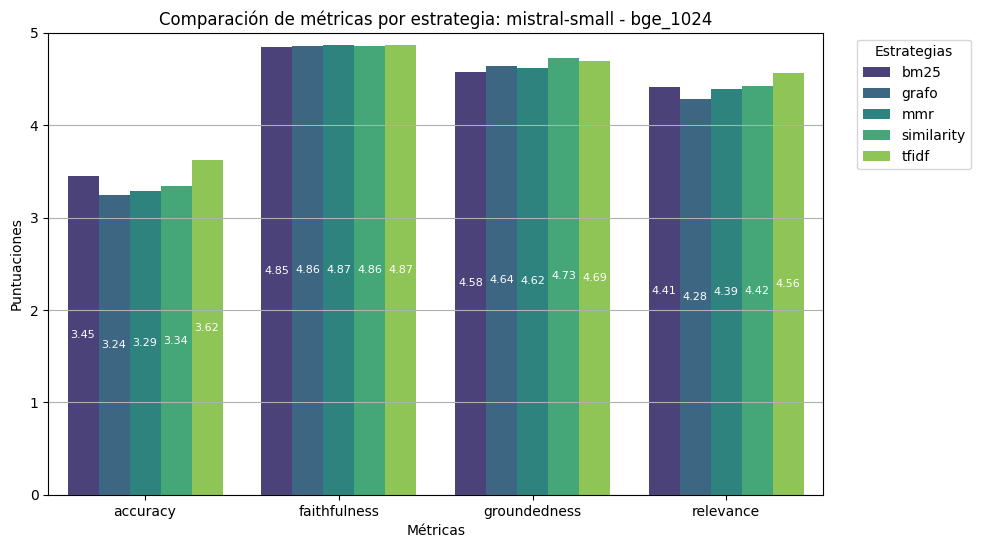
\includegraphics[width=1\textwidth]{imagenes/0128_bge_1024.png}
	    				\caption{Sin reranking}
	    			\end{subfigure}   
	    			\begin{subfigure}{.49\textwidth}
	    				\centering
	    				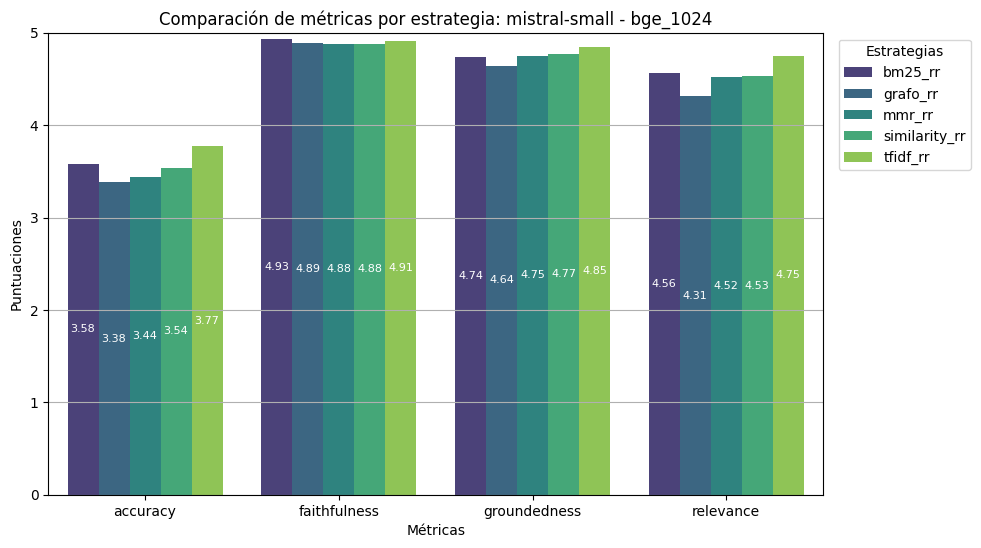
\includegraphics[width=1\textwidth]{imagenes/0128_bge_rr_1024.png}
	    				\caption{Con reranking}
	    			\end{subfigure} 			
	    			\caption{Gráfica de rendimiento del modelo Mistral Small 3.2 usando el modelo de embedding BGE-M3 y tamaños de documento 1024}
	    			\label{fig:0128_bge_1024}       
	    		\end{figure} 
	    		
	    		\begin{figure}[H]
	    			\centering
	    			\begin{subfigure}{.49\textwidth}
	    				\centering
	    				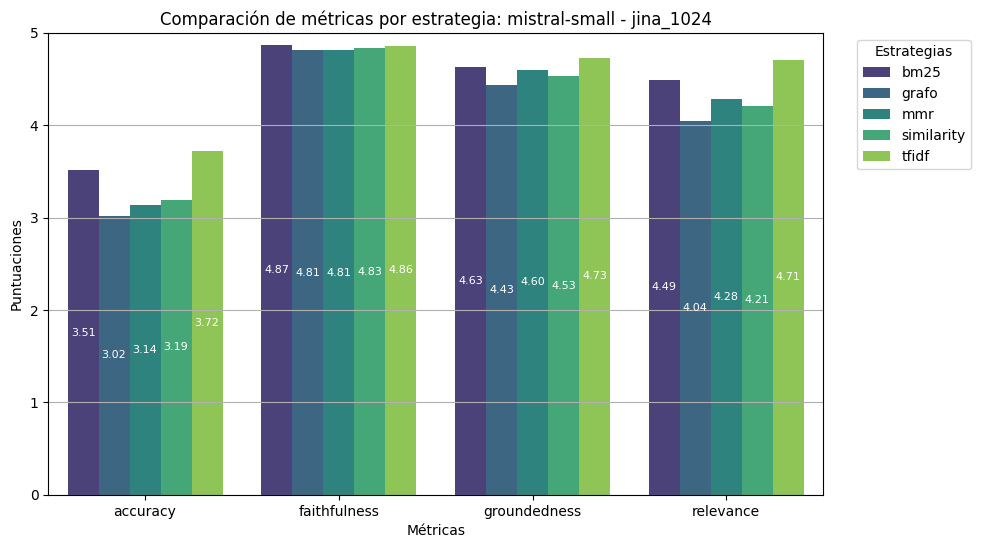
\includegraphics[width=1\textwidth]{imagenes/0129_jina_1024.png}
	    				\caption{Sin reranking}
	    			\end{subfigure}   
	    			\begin{subfigure}{.49\textwidth}
	    				\centering
	    				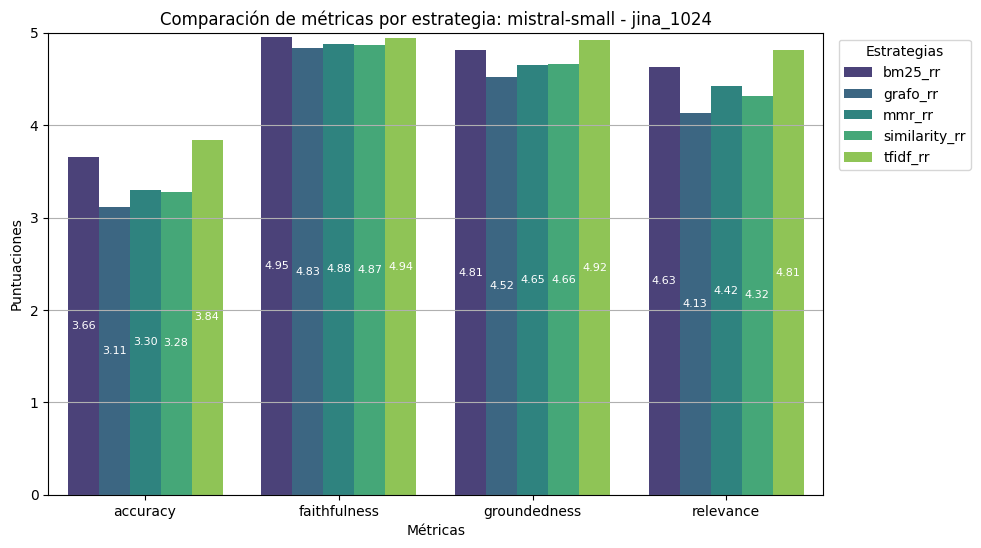
\includegraphics[width=1\textwidth]{imagenes/0129_jina_rr_1024.png}
	    				\caption{Con reranking}
	    			\end{subfigure} 			
	    			\caption{Gráfica de rendimiento del modelo Mistral Small 3.2 usando el modelo de embedding JINA y tamaños de documento 1024}
	    			\label{fig:0129_jina_1024}       
	    		\end{figure} 
	    		
	    		\begin{figure}[H]
	    			\centering
	    			\begin{subfigure}{.49\textwidth}
	    				\centering
	    				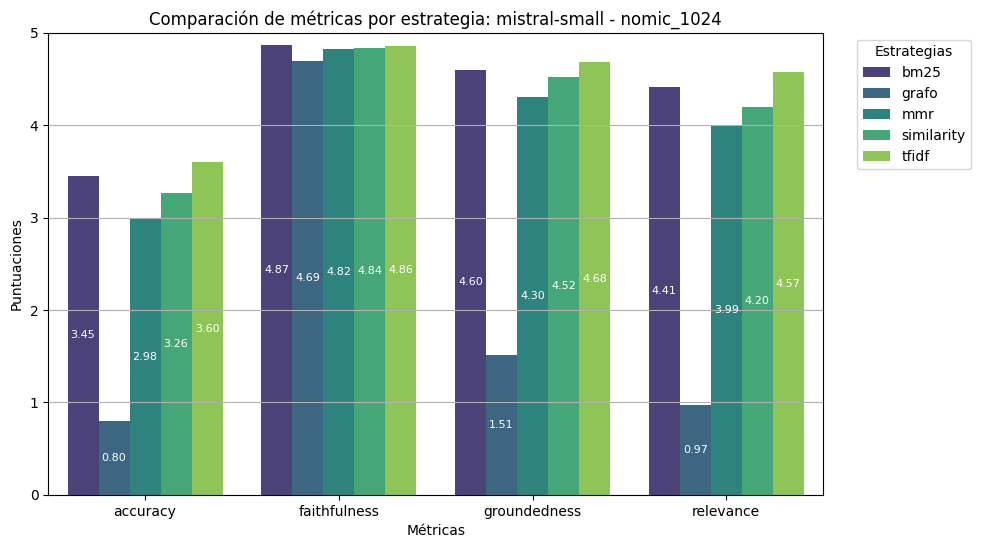
\includegraphics[width=1\textwidth]{imagenes/0130_nomic_1024.png}
	    				\caption{Sin reranking}
	    			\end{subfigure}   
	    			\begin{subfigure}{.49\textwidth}
	    				\centering
	    				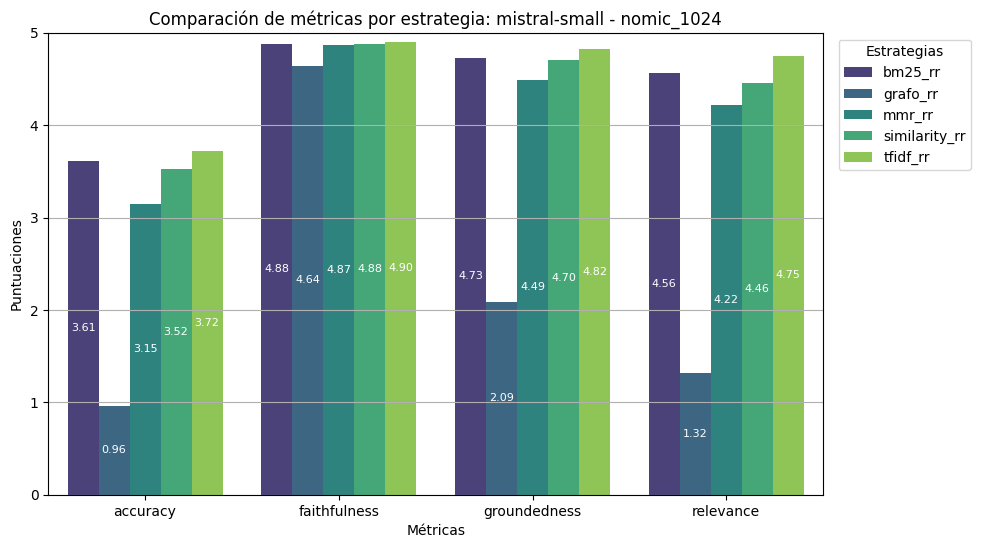
\includegraphics[width=1\textwidth]{imagenes/0130_nomic_rr_1024.png}
	    				\caption{Con reranking}
	    			\end{subfigure} 			
	    			\caption{Gráfica de rendimiento del modelo Mistral Small 3.2 usando el modelo de embedding Nomic-Embed-Text y tamaños de documento 1024}
	    			\label{fig:0130_nomic_1024}       
	    		\end{figure} 
	    		
	    		\begin{figure}[H]
	    			\centering
	    			\begin{subfigure}{.49\textwidth}
	    				\centering
	    				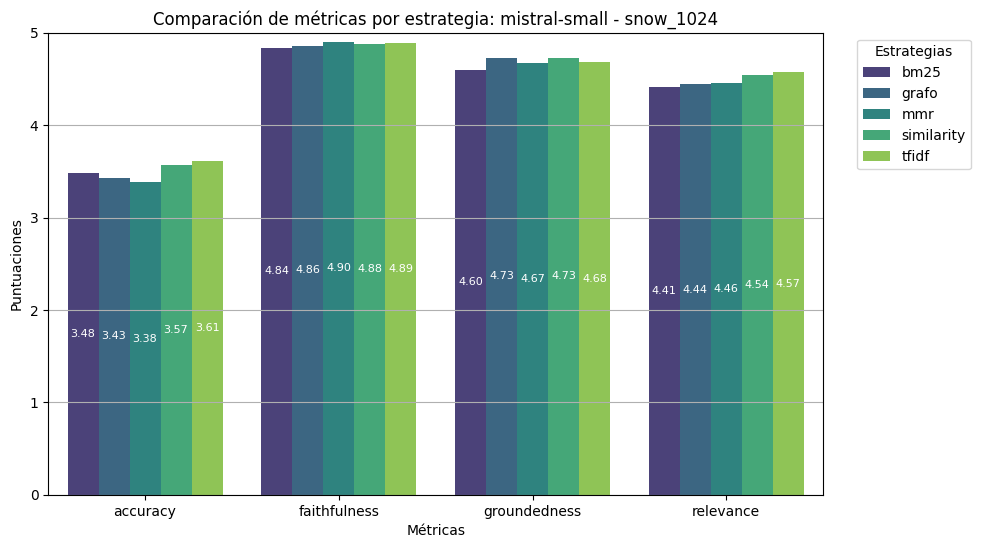
\includegraphics[width=1\textwidth]{imagenes/0131_snow_1024.png}
	    				\caption{Sin reranking}
	    			\end{subfigure}   
	    			\begin{subfigure}{.49\textwidth}
	    				\centering
	    				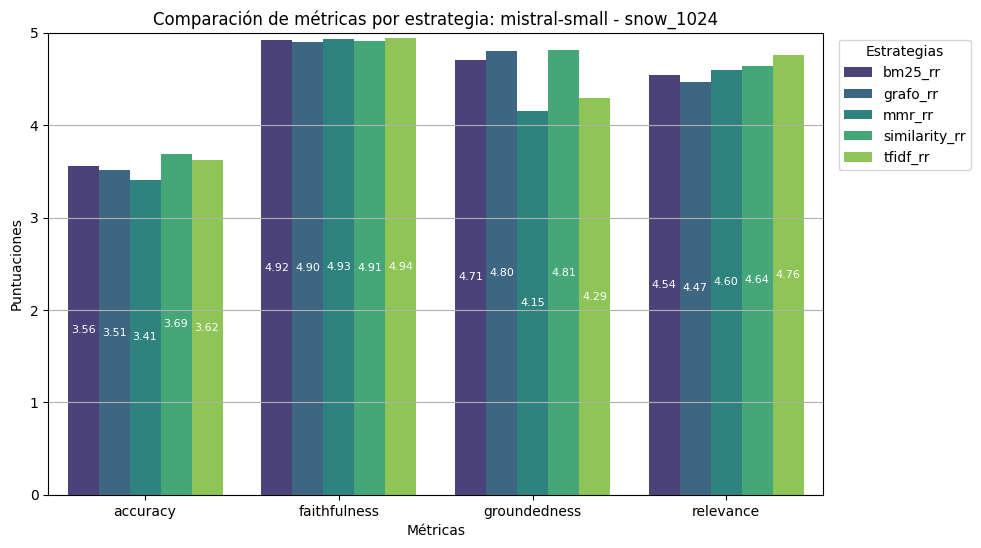
\includegraphics[width=1\textwidth]{imagenes/0131_snow_rr_1024.png}
	    				\caption{Con reranking}
	    			\end{subfigure} 			
	    			\caption{Gráfica de rendimiento del modelo Mistral Small 3.2 usando el modelo de embedding Snowflakev2 y tamaños de documento 1024}
	    			\label{fig:0131_snow_1024}       
	    		\end{figure} 	
	    		
	    	\subsubsection{Resultados usando un prompt modificado en bases de datos con tamaño de documentos 1024}
	    	
	    		En esta tanda de pruebas se hizo una modificación en el \textit{prompt} interno del sistema RAG. En este \textit{prompt} (figura  \ref{fig:0138_prompt_mejora}), se indica que debe efectuar una respuesta de forma más simple y escueta a la consulta del usuario. El \textit{prompt} por defecto se extiende demasiado en su respuesta, generando estructuras y listas que pueden afectar negativamente a la evaluación del \textit{accuracy}.    		
	    		
	    		\begin{figure}[H]
	    			\centering
	    			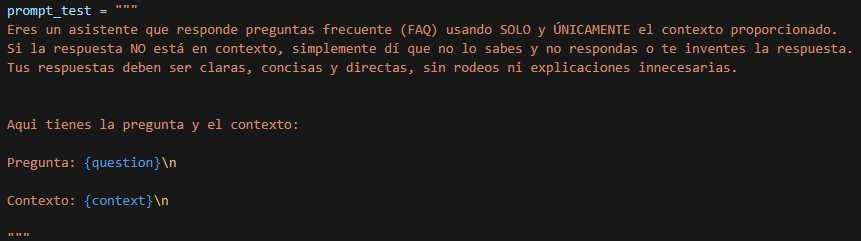
\includegraphics[width=1\textwidth]{imagenes/0138_prompt_mejora.png}
	    			\caption{Modificación hecha en el prompt}		
	    			\label{fig:0138_prompt_mejora}
	    		\end{figure} 
	    			    		
	    		\noindent Los resultados se muestran en la siguiente tabla:
	    	
	    		\newpage
		    	\begin{table}[H]
		    		\centering
		    		\tiny
		    		\begin{tblr}{
		    				row{1} = {bg=white}, 
		    				row{2-11} = {bg=yellow!20}, 
		    				row{12-21} = {bg=green!20},    				
		    				row{22-31} = {bg=blue!20}, 
		    				row{32-41} = {bg=violet!20}, 
		    				hlines,
		    				vlines,
		    			}
		    			\textbf{Embedding} & \textbf{Estrategia} & \textbf{Accuracy} & \textbf{Faithfulness} & \textbf{Groundedness} & \textbf{Relevance} \\
		    			bge-m3 & tfidf\_rr & \SetCell{bg=yellow}\textbf{3.72} & \SetCell{bg=yellow}\textbf{4.95} & \SetCell{bg=yellow}\textbf{4.4} & \SetCell{bg=yellow}\textbf{4.82} \\
		    			bge-m3 & bm25\_rr & 3.51 & 4.8 & 4.24 & 4.64 \\
		    			bge-m3 & similarity\_rr & 3.44 & 4.77 & 4.09 & 4.55 \\
		    			bge-m3 & tfidf & 3.43 & 4.83 & 4.07 & 4.67 \\
		    			bge-m3 & bm25 & 3.38 & 4.82 & 3.98 & 4.52 \\
		    			bge-m3 & mmr\_rr & 3.32 & 4.86 & 4.09 & 4.51 \\
		    			bge-m3 & grafo\_rr & 3.21 & 4.74 & 3.96 & 4.31 \\
		    			bge-m3 & similarity & 3.12 & 4.74 & 3.84 & 4.38 \\
		    			bge-m3 & mmr & 3.04 & 4.83 & 3.9 & 4.37 \\
		    			bge-m3 & grafo & 2.95 & 4.76 & 3.76 & 4.27 \\
		    			jina & tfidf\_rr & \SetCell{bg=green}\textbf{3.66} & \SetCell{bg=green}\textbf{4.92} & \SetCell{bg=green}\textbf{4.3} & \SetCell{bg=green}\textbf{4.73} \\
		    			jina & bm25\_rr & 3.55 & 4.9 & 4.26 & 4.66 \\
		    			jina & bm25 & 3.46 & 4.79 & 4.01 & 4.56 \\
		    			jina & tfidf & 3.37 & 4.81 & 3.97 & 4.57 \\
		    			jina & mmr\_rr & 3.1 & 4.87 & 3.98 & 4.41 \\
		    			jina & similarity\_rr & 3.09 & 4.77 & 3.91 & 4.37 \\
		    			jina & similarity & 2.84 & 4.72 & 3.74 & 4.22 \\
		    			jina & mmr & 2.81 & 4.88 & 3.66 & 4.26 \\
		    			jina & grafo\_rr & 2.77 & 4.53 & 3.52 & 4.12 \\
		    			jina & grafo & 2.6 & 4.48 & 3.38 & 4.06 \\
		    			nomic & tfidf\_rr & \SetCell{bg=blue!50}\textbf{3.67} & \SetCell{bg=blue!50}\textbf{4.91} & \SetCell{bg=blue!50}\textbf{4.3} & \SetCell{bg=blue!50}\textbf{4.75} \\
		    			nomic & bm25\_rr & 3.39 & 4.87 & 4.08 & 4.56 \\
		    			nomic & tfidf & 3.38 & 4.76 & 3.95 & 4.55 \\
		    			nomic & bm25 & 3.23 & 4.84 & 3.81 & 4.4 \\
		    			nomic & similarity\_rr & 3.14 & 4.75 & 3.77 & 4.36 \\
		    			nomic & mmr\_rr & 2.95 & 4.79 & 3.65 & 4.24 \\
		    			nomic & similarity & 2.9 & 4.7 & 3.44 & 4.04 \\
		    			nomic & grafo\_rr & 2.77 & 4.67 & 3.44 & 3.97 \\
		    			nomic & mmr & 2.62 & 4.85 & 3.15 & 3.99 \\
		    			nomic & grafo & 2.56 & 4.53 & 3.22 & 3.8 \\
		    			snowflake & tfidf\_rr & \SetCell{bg=violet!50}\textbf{3.65} & \SetCell{bg=violet!50}\textbf{4.92} & \SetCell{bg=violet!50}\textbf{4.27} & \SetCell{bg=violet!50}\textbf{4.75} \\
		    			snowflake & similarity\_rr & 3.53 & 4.87 & 4.24 & 4.62 \\
		    			snowflake & mmr\_rr & 3.44 & 4.89 & 4.16 & 4.62 \\
		    			snowflake & tfidf & 3.43 & 4.81 & 3.99 & 4.57 \\
		    			snowflake & similarity & 3.4 & 4.86 & 4.08 & 4.54 \\
		    			snowflake & grafo\_rr & 3.36 & 4.77 & 4.09 & 4.47 \\
		    			snowflake & bm25\_rr & 3.35 & 4.91 & 4.09 & 4.57 \\
		    			snowflake & grafo & 3.22 & 4.76 & 3.9 & 4.4 \\
		    			snowflake & bm25 & 3.21 & 4.79 & 3.79 & 4.4 \\
		    			snowflake & mmr & 3.17 & 4.95 & 3.97 & 4.51 \\
		    			
		    		\end{tblr}
		    		\caption{Resultados de Mistral Small 3.2 en embeddings 1024 de tamaño de documentos y el prompt modificado}
		    		\label{tab:result_mistral_1024++}
		    	\end{table}
		    	
		    	\noindent A la vista de los resultados obtenidos de estas pruebas, podemos asegurar que la modificación del \textit{prompt} introducida ha tenido influencia en ellos. La mejora esperada no se ha producido, y hemos tenido resultados más bajos que en el apartado anterior en todas las métricas salvo en \textit{faithfulness}.
		    	
		    	\noindent La simplificación del \textit{prompt} de la cual esperábamos mejores resultados, ha afectado negativamente a estos. El dato positivo que podemos extraer de esta batería de pruebas es que al modificar el \textit{prompt}, obtenemos una respuesta diferente del modelo de lenguaje, y por consiguiente, unos resultados distintos para nuestros test.
		    	
		    	\noindent Resultados que se pueden observar individualmente (como en los demás apartados), en las siguientes gráficas:
		    			    	
		    	\begin{figure}[H]
		    		\centering
		    		\begin{subfigure}{.49\textwidth}
		    			\centering
		    			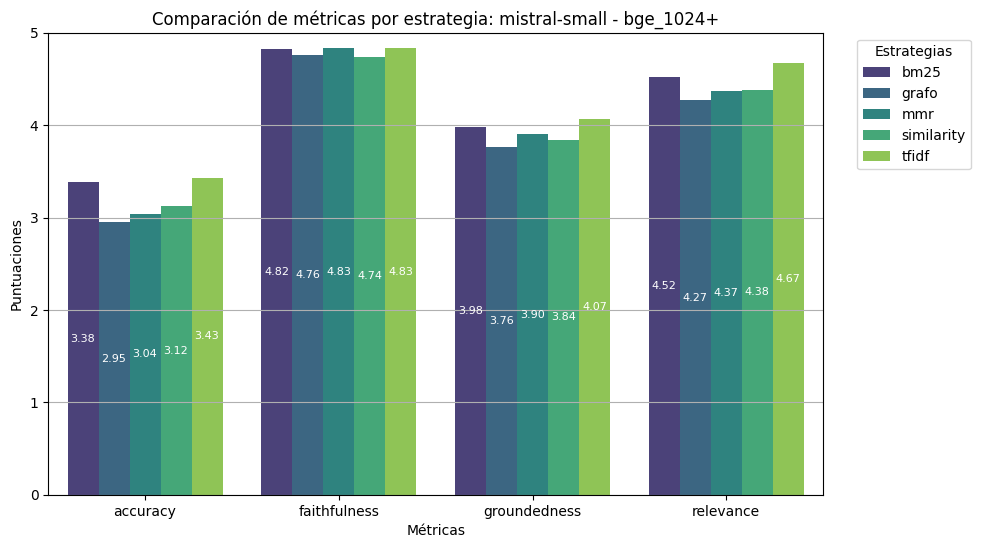
\includegraphics[width=1\textwidth]{imagenes/0132_bge+_1024.png}
		    			\caption{Sin reranking}
		    		\end{subfigure}   
		    		\begin{subfigure}{.49\textwidth}
		    			\centering
		    			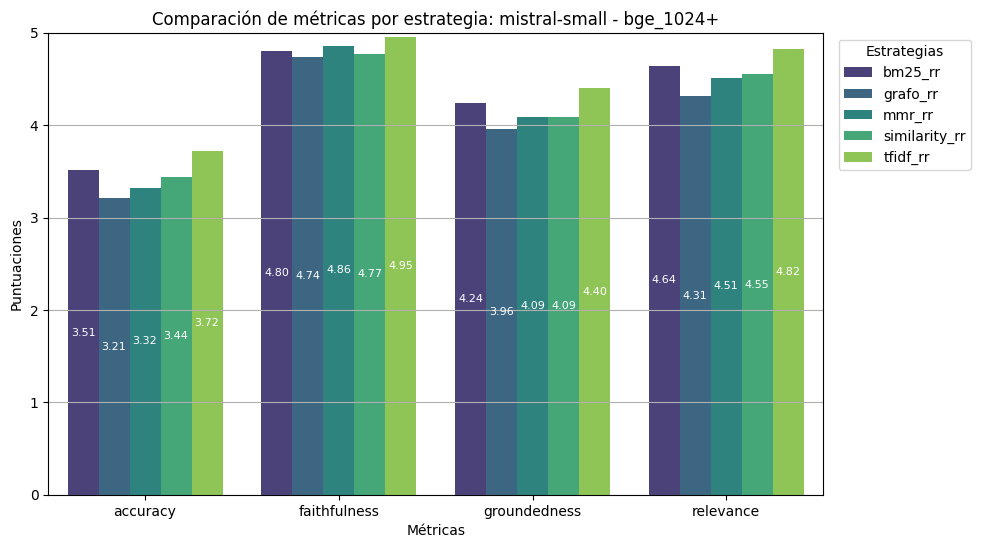
\includegraphics[width=1\textwidth]{imagenes/0132_bge+_rr_1024.png}
		    			\caption{Con reranking}
		    		\end{subfigure} 			
		    		\caption{Gráfica de rendimiento del modelo Mistral Small 3.2 usando el modelo de embedding BGE-M3, tamaños de documento 1024 y el prompt modificado}
		    		\label{fig:0132_bge+_1024}       
		    	\end{figure} 
		    	
		    	\begin{figure}[H]
		    		\centering
		    		\begin{subfigure}{.49\textwidth}
		    			\centering
		    			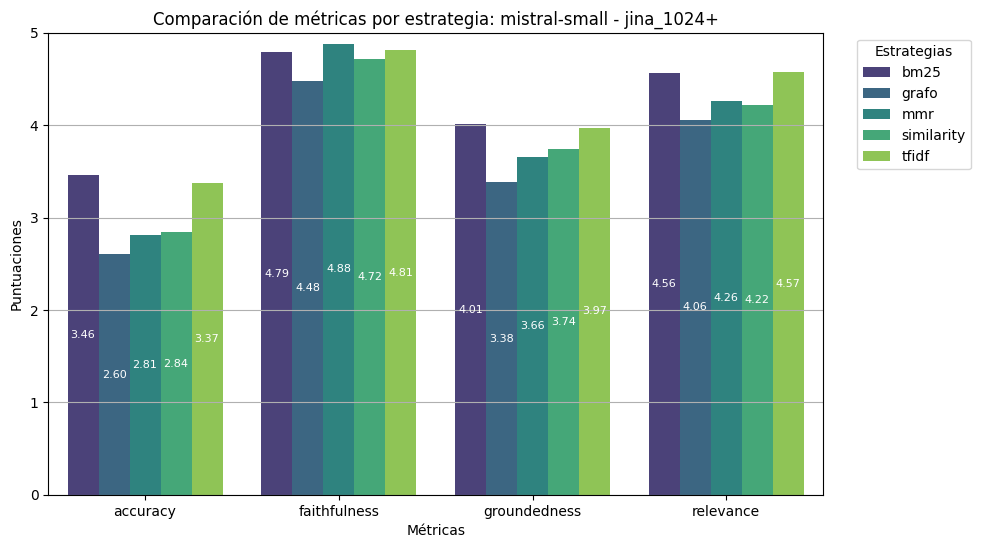
\includegraphics[width=1\textwidth]{imagenes/0133_jina+_1024.png}
		    			\caption{Sin reranking}
		    		\end{subfigure}   
		    		\begin{subfigure}{.49\textwidth}
		    			\centering
		    			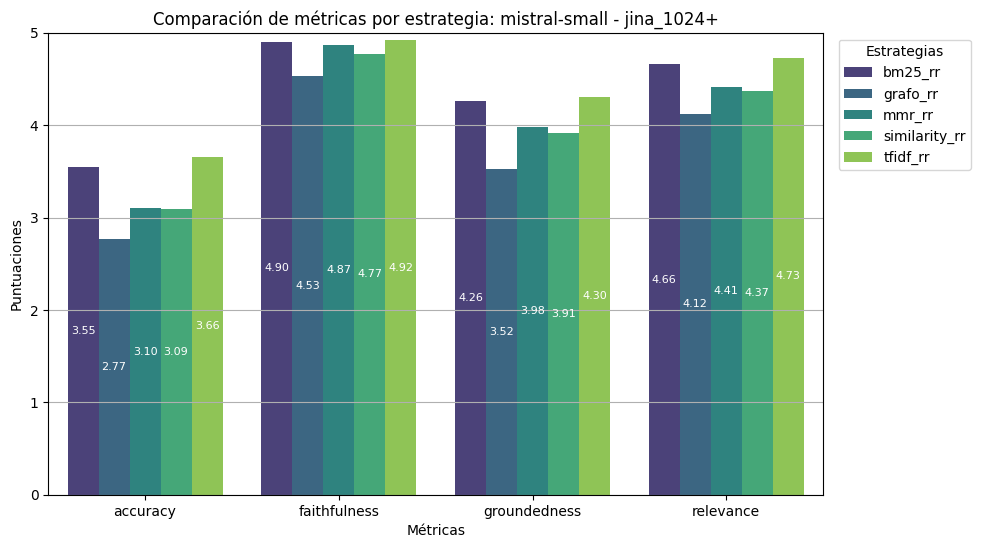
\includegraphics[width=1\textwidth]{imagenes/0133_jina+_rr_1024.png}
		    			\caption{Con reranking}
		    		\end{subfigure} 			
		    		\caption{Gráfica de rendimiento del modelo Mistral Small 3.2 usando el modelo de embedding JINA, tamaños de documento 1024 y el prompt modificado}
		    		\label{fig:0133_jina+_1024}       
		    	\end{figure} 
		    	
		    	\begin{figure}[H]
		    		\centering
		    		\begin{subfigure}{.49\textwidth}
		    			\centering
		    			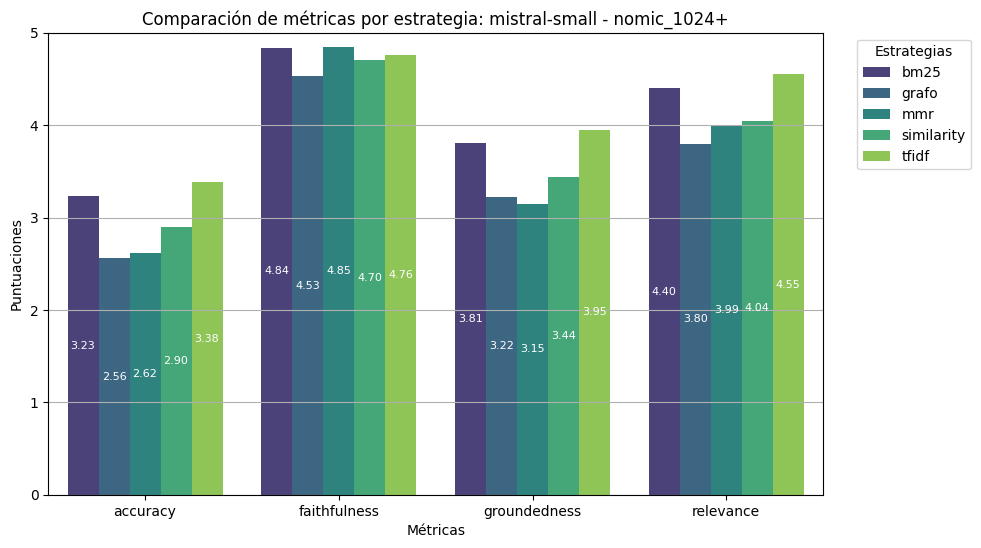
\includegraphics[width=1\textwidth]{imagenes/0134_nomic+_1024.png}
		    			\caption{Sin reranking}
		    		\end{subfigure}   
		    		\begin{subfigure}{.49\textwidth}
		    			\centering
		    			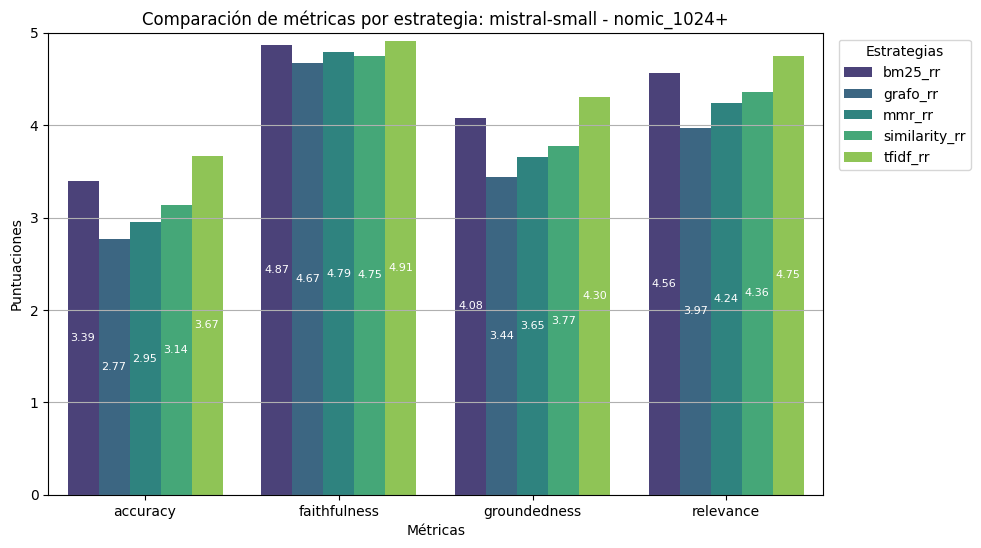
\includegraphics[width=1\textwidth]{imagenes/0134_nomic+_rr_1024.png}
		    			\caption{Con reranking}
		    		\end{subfigure} 			
		    		\caption{Gráfica de rendimiento del modelo Mistral Small 3.2 usando el modelo de embedding Nomic-Embed-Text, tamaños de documento 1024 y el prompt modificado}
		    		\label{fig:0134_nomic+_1024}       
		    	\end{figure} 
		    	
		    	\begin{figure}[H]
		    		\centering
		    		\begin{subfigure}{.49\textwidth}
		    			\centering
		    			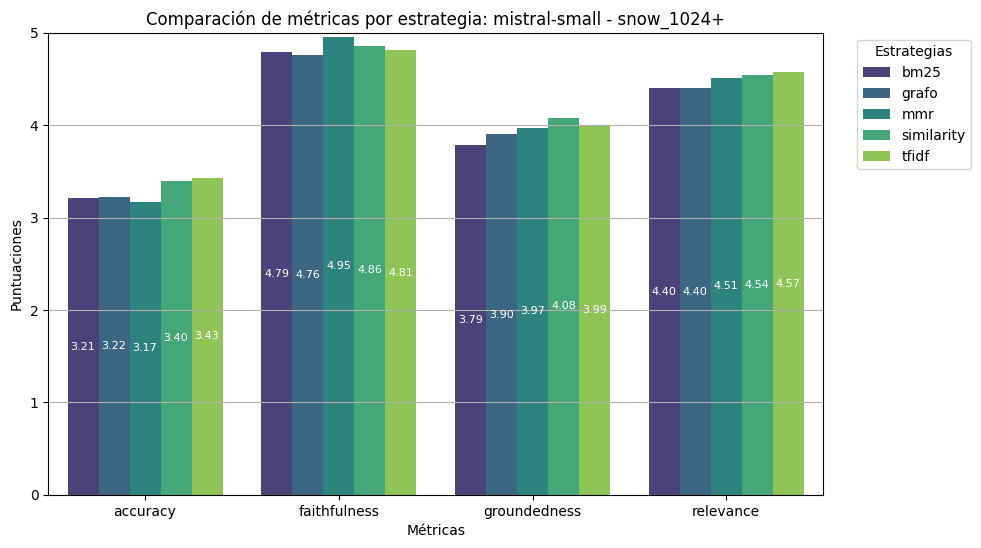
\includegraphics[width=1\textwidth]{imagenes/0135_snow+_1024.png}
		    			\caption{Sin reranking}
		    		\end{subfigure}   
		    		\begin{subfigure}{.49\textwidth}
		    			\centering
		    			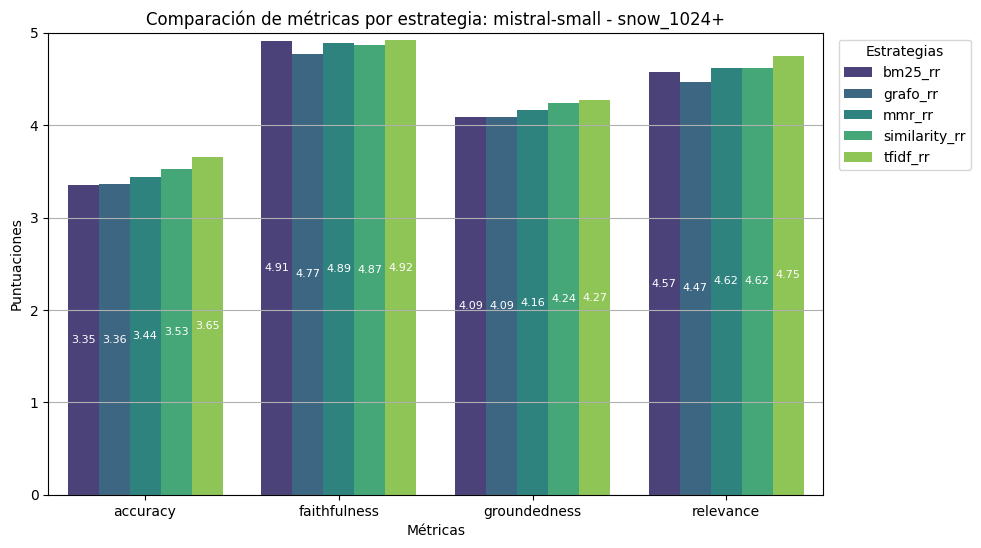
\includegraphics[width=1\textwidth]{imagenes/0135_snow+_rr_1024.png}
		    			\caption{Con reranking}
		    		\end{subfigure} 			
		    		\caption{Gráfica de rendimiento del modelo Mistral Small 3.2 usando el modelo de embedding Snowflakev2, tamaños de documento 1024 y el prompt modificado}
		    		\label{fig:0135_snow+_1024}       
		    	\end{figure} 	
		    	  	
    	\subsection{Resultados de Llama 3.2}
    	
    		\textit{Llama 3.2} es el modelo usado para realizar estas pruebas de forma local. Este modelo es el más modesto de los utilizados en el proyecto, contando solo con 3 billones (ingleses) de parámetros. Debido a esto, se espera recibir unos resultados peores a los anteriores mostrados.
    		
    		\noindent Otro factor importante derivado del método de ejecución de este modelo es que, al ser ejecutado localmente, consume bastante tiempo en generar una respuesta. Al depender de la configuración de la máquina donde se use, si esta no cumple con los requisitos necesarios los tiempos de respuesta se alargan considerablemente. En nuestro caso, al no disponer de una tarjeta gráfica \textit{nvidia}, sufrimos esta consecuencia.
    		
    		\noindent Para mitigar la tardanza en el tiempo de respuesta, se planteó usar un 10\% del conjunto de preguntas (unas 30) y extrapolar los resultados. Dichos resultados se obtuvieron en una media de 3 horas y 20 minutos para cada prueba, empleándose alrededor de unas 16 horas y 40 minutos para realizar las pruebas en un solo embedding con la suma de todas las estrategias de búsqueda.
    		
    		\noindent Los resultados obtenidos para un solo embedding se muestran en la siguiente tabla:
    		
    		\begin{table}[H]
    			\centering
    			\tiny
    			\begin{tblr}{
    					row{1} = {bg=white}, 
    					row{2-11} ={bg=green!20},    
    					hlines,
    					vlines,
    				}
    				\textbf{Embedding} & \textbf{Estrategia} & \textbf{Accuracy} & \textbf{Faithfulness} & \textbf{Groundedness} & \textbf{Relevance} \\
    				jina & similarity\_rr & \SetCell{bg=green}\textbf{3.08} & 4.17 & \SetCell{bg=green}\textbf{3.75} & 4.25 \\
    				jina & grafo & 2.94 & 4.29 & 3.18 & 4.18 \\
    				jina & similarity & 2.76 & 3.94 & 3.41 & 4.24 \\
    				jina & tfidf\_rr & 2.5 & \SetCell{bg=green}\textbf{4.5} & 3.33 & \SetCell{bg=green}\textbf{4.67} \\
    				jina & tfidf & 2.4 & 4.0 & 3.47 & 4.33 \\
    				jina & bm25\_rr & 2.36 & 4.18 & 3.0 & 4.36 \\
    				jina & grafo\_rr & 2.3 & 4.4 & 3.2 & 4.6 \\
    				jina & mmr & 2.29 & 4.29 & 3.43 & 3.86 \\
    				jina & mmr\_rr & 1.8 & 4.1 & 3.4 & 3.9 \\
    				jina & bm25 & 1.76 & 3.94 & 3.0 & 4.53 \\
    				
    			\end{tblr}
    			\caption{Resultados de Llama 3.2 en embeddings 1024 de tamaño de documentos}
    			\label{tab:result_llama}
    		\end{table}
    		
    		\noindent Y como se esperaba, se obtienen los peores resultados en todas las métricas. Destaca la pobre puntuación obtenida en el \textit{accuracy} en la mayoría de los agentes, algunos no llegan a superar el 50\%. Siendo la mejor puntuación de esta, casi 8 décimas peor que el mejor modelo, esta claro que no es un modelo aconsejable para el uso. 
    		
    		\noindent Aunque las demás métricas consiguen resultados más o menos decentes, siguen estando muy por debajo de las mejores puntuaciones obtenidas.
    		
    		\noindent No se ha decidido usar otro modelo de embedding por los malos resultados obtenidos usando \textit{JINA}, el mejor modelo en comparación vistas las otras tablas de pruebas.
    		
    		\noindent En las siguientes figuras, se muestra de forma gráfica los resultados presentes en la tabla \ref{tab:result_llama}.
    		
    		\begin{figure}[H]
    			\centering
    			\begin{subfigure}{.49\textwidth}
    				\centering
    				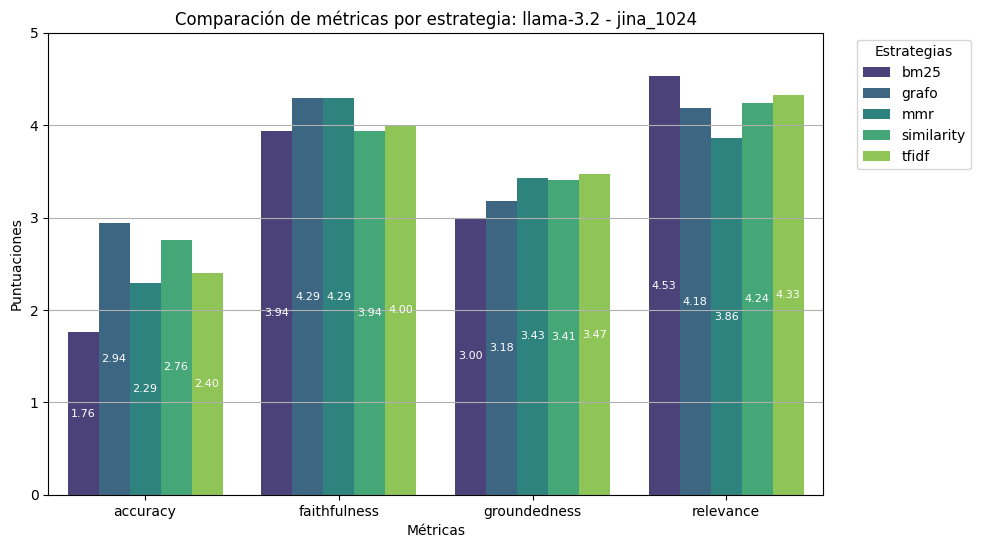
\includegraphics[width=1\textwidth]{imagenes/0136_llama_jina.png}
    				\caption{Sin reranking}
    			\end{subfigure}   
    			\begin{subfigure}{.49\textwidth}
    				\centering
    				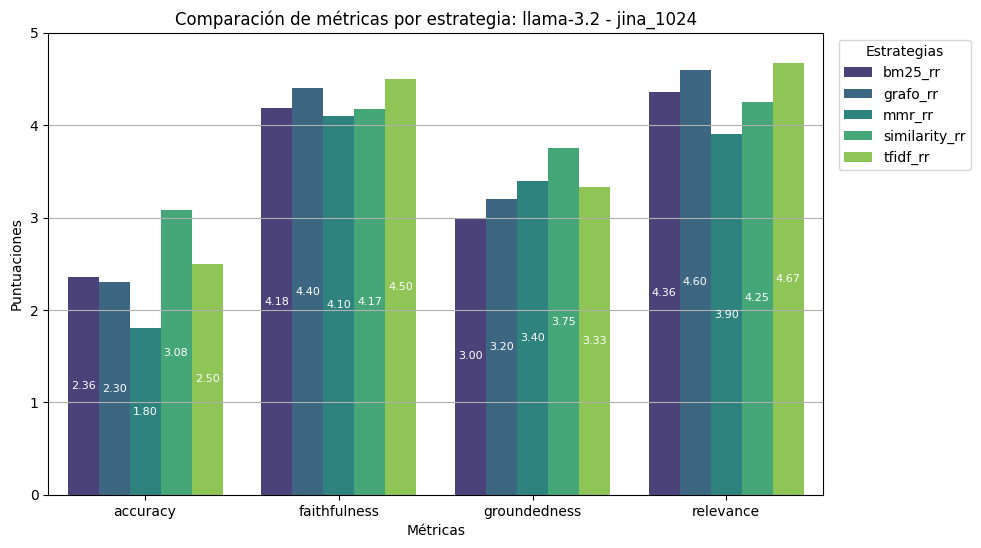
\includegraphics[width=1\textwidth]{imagenes/0136_llama_jina_rr.png}
    				\caption{Con reranking}
    			\end{subfigure} 			
    			\caption{Gráfica de rendimiento del modelo Llama 3.2 usando el modelo de embedding Jina y tamaños de documento 1024}
    			\label{fig:0136_llama_jina}       
    		\end{figure} 
    	
    	\subsection{Resultados de GPT-4.1}
    	
    		El modelo \textit{GPT-4.1} es el último usado en las pruebas definidas en nuestro proyecto. Este modelo perteneciente a \textit{OpenAI} es de pago, por lo que hay que controlar el uso que le pedimos a esta plataforma si no queremos gastar mucho dinero. Por este motivo se redujo el conjunto de pruebas a un 25\% del total (75 preguntas) para después extrapolar los resultados conseguidos.
    		
    		\noindent A su vez, el modelo de embedding utilizado para las pruebas también comparte plataforma con este modelo de lenguaje. Se optó por probar ambos, para medir el rendimiento de los modelos de pago en comparación al resto. El modelo de embedding (\textit{text-embedding-3-small}) fue configurado para usar documentos de tamaño 1024.
    		
    		\noindent El tiempo para obtener los resultados fue de 40 minutos por modelo de embedding. Teniendo en cuenta que obtenemos los resultados sin y con \textit{reranking} en la misma prueba, se produjeron cinco ejecuciones en un total de dos horas y media, con un costo aproximado de 15 dólares.
    		
    		\noindent\textbf{Nota:} Cada consulta hecha generaba alrededor de 3000 tokens, y su coste era de 0,01\$.
    		
    		\noindent Los resultados de las pruebas son los mostrados en la siguiente tabla:
    		
    		\begin{table}[H]
    			\centering
    			\tiny
    			\begin{tblr}{
    					row{1} = {bg=white}, 
    					row{2-11} ={bg=violet!20},    
    					hlines,
    					vlines,
    				}
    				\textbf{Embedding} & \textbf{Estrategia} & \textbf{Accuracy} & \textbf{Faithfulness} & \textbf{Groundedness} & \textbf{Relevance} \\
    				text-embedding-3-small & tfidf & \SetCell{bg=violet!50}\textbf{4.32} & \SetCell{bg=violet!50}\textbf{4.95} & 4.91 & 4.68 \\
    				text-embedding-3-small & tfidf\_rr & 4.27 & 4.92 & \SetCell{bg=violet!50}\textbf{4.96} & \SetCell{bg=violet!50}\textbf{4.75} \\
    				text-embedding-3-small & similarity\_rr & 3.96 & 4.89 & 4.88 & 4.41 \\
    				text-embedding-3-small & similarity & 3.95 & 4.88 & 4.89 & 4.49 \\
    				text-embedding-3-small & mmr\_rr & 3.92 & 4.89 & 4.88 & 4.59 \\
    				text-embedding-3-small & bm25 & 3.83 & 4.91 & 4.88 & 4.45 \\
    				text-embedding-3-small & bm25\_rr & 3.83 & 4.92 & 4.95 & 4.41 \\
    				text-embedding-3-small & grafo\_rr & 3.68 & 4.91 & 4.85 & 4.19 \\
    				text-embedding-3-small & grafo & 3.67 & 4.87 & 4.81 & 4.17 \\
    				text-embedding-3-small & mmr & 3.6 & 4.87 & 4.81 & 4.28 \\
    			\end{tblr}
    			\caption{Resultados de GPT-4.1 en embeddings 1024 de tamaño de documentos}
    			\label{tab:result_gpt}
    		\end{table}
    		
    		\noindent Como se puede apreciar en la tabla anterior, los resultados obtenidos son los mejores obtenidos hasta ahora, con la única excepción de la métrica de relevancia. 
    		
    		\noindent En el caso del \textit{accuracy}, las estrategias \textit{TF-IDF} sin y con \textit{reranking} superan los 4.25 de puntuación, lo cual indica una respuesta muy parecida a la esperada. Para las demás estrategias, el \textit{accuracy} siempre supera a la mejor obtenida anteriormente. 
    		
    		\noindent Las métricas \textit{faithfulness} y \textit{groundedness} se mantienen muy altas, rozando el 5 en las mejores y siempre superando la puntuación mínima de 4.8. Es una buena manera de saber que, con estos modelos se utiliza muy bien el contexto recuperado para generar las respuestas.
    		
    		\noindent En cuanto a la relevancia, aún no siendo el valor más alto obtenido en estas pruebas, el mejor conseguido sigue manteniendo una puntuación muy alta (4.75). A excepción de algunas estrategias, las puntuaciones obtenidas en esta métrica son generalmente muy altas.
    		
    		\noindent En las siguientes figuras, podemos ver el contenido de la tabla \ref{tab:result_gpt} de forma gráfica.
    		
    		\begin{figure}[H]
    			\centering
    			\begin{subfigure}{.49\textwidth}
    				\centering
    				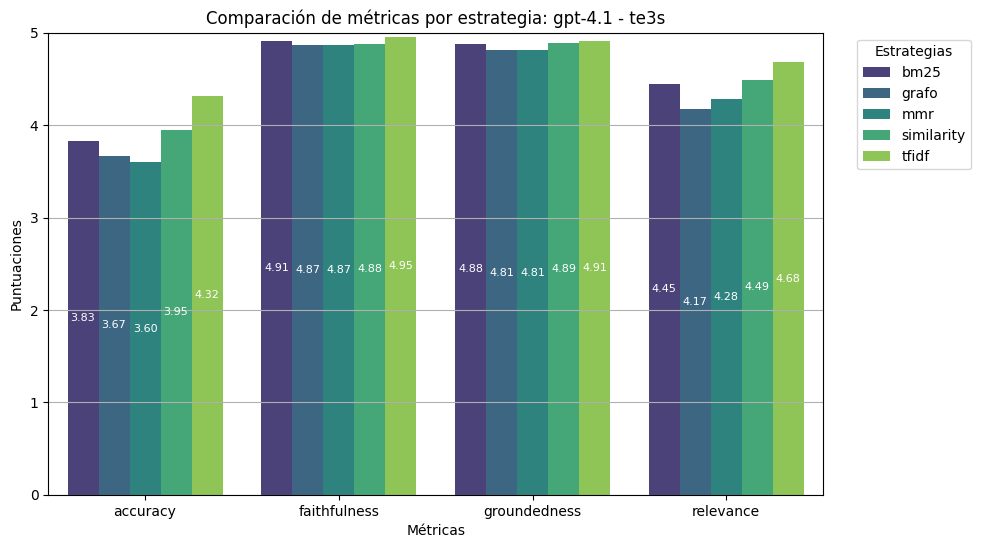
\includegraphics[width=1\textwidth]{imagenes/0137_gpt_te3s.png}
    				\caption{Sin reranking}
    			\end{subfigure}   
    			\begin{subfigure}{.49\textwidth}
    				\centering
    				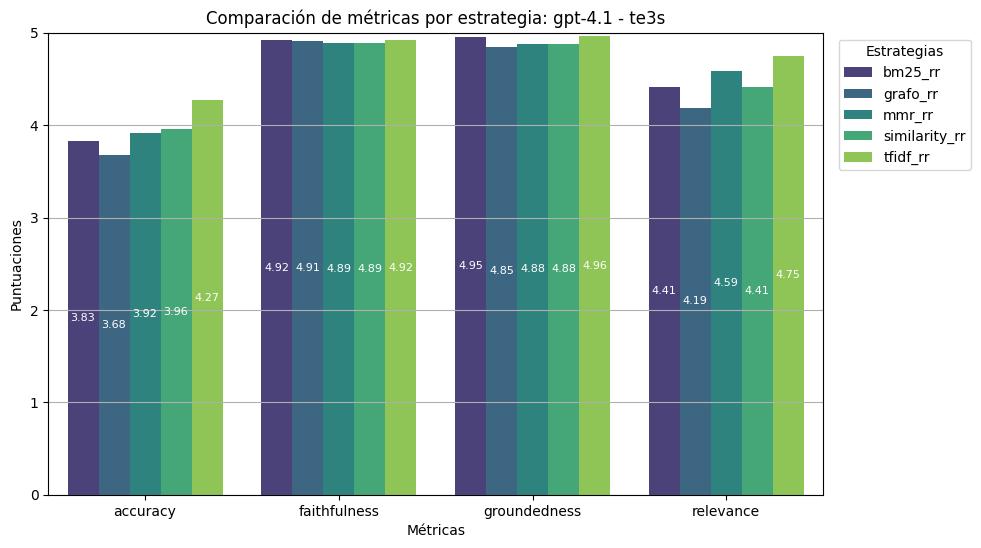
\includegraphics[width=1\textwidth]{imagenes/0137_gpt_te3s_rr.png}
    				\caption{Con reranking}
    			\end{subfigure} 			
    			\caption{Gráfica de rendimiento del modelo GPT-4.1 usando el modelo de embedding text-embedding-3-small y tamaños de documento 1024}
    			\label{fig:0137_gpt_te3s}       
    		\end{figure} 
    		
   	\section{Conclusión sobre los resultados}
   	
   		Tras realizar las pruebas y, habiendo consultado los resultados; podemos concluir aportando el conocimiento adquirido de estos. Para ello, vamos a responder una lista de preguntas relacionadas con el rendimiento del RAG ante cambios o modificaciones en su configuración. Y como colofón, explicaremos las deducciones finales obtenidas sobre los resultados.
   		
   		%\subsection{Preguntas sobre los resultados}
   		
	   		\noindent\textbf{¿Cómo afecta el tamaño del LLM a la calidad de la respuesta en un sistema RAG?} Los modelos de lenguaje más grandes (con mayor número de parámetros) obtienen mejores resultados. Los resultados obtenidos por \textit{Llama 3.2} (tabla \ref{tab:result_llama}) son inferiores a los otros dos modelos de lenguaje (tablas \ref{tab:result_mistral_1024} y \ref{tab:result_gpt}). Esto se debe al tamaño de los modelos, Llama 3.2 (3B) es mucho más pequeño que \textit{Mistral Small 3.2} (24B) y \textit{GPT-4.1} (desconocido, aunque sabemos que la versión GPT3 cuenta con 175B de parámetros). Por lo tanto, podemos asegurar que conseguiremos mejores respuestas con modelos más grandes.
	   		
	   		\noindent\textbf{¿Pueden diferencias sutiles en el prompt afectar significativamente la alineación de la recuperación y la generación?} En nuestro caso, solo afecta a la generación de respuesta, ya que la recuperación no se utiliza un \textit{prompt} (recupera documentos relevantes a la consulta). En la prueba realizada modificando el \textit{prompt} (tabla \ref{tab:result_mistral_1024++}), pedimos una respuesta más simple y escueta, y los resultados consecuente fueron peores a los conseguidos anteriormente. Debido a esto, concluimos que el \textit{prompt} usado por defecto es mejor generando una respuesta más parecida a la esperada y, que la modificación de este influye en los resultados.
	   		
	   		\noindent\textbf{¿Cómo impacta el tamaño del fragmento de documento recuperado en la calidad de la respuesta?} Hemos comprobado este factor en las dos primeras tandas de pruebas (tablas \ref{tab:result_mistral_512} y \ref{tab:result_mistral_1024}). Los resultados obtenidos muestran que un tamaño mayor es mejor para generar una respuesta. Así que, podemos decir que la respuesta generada se ve favorecida si dispone de documentos recuperados con un mayor tamaño de contexto.
	   		
	   		\noindent\textbf{¿Cómo impacta el tamaño de la base de conocimiento en el rendimiento general?} Hemos trabajado con bases de conocimiento que oscilaban entre 45MB y 65MB, por lo que no hemos apreciado diferencias considerables en el tiempo de recuperación de documentos. Este tiempo era casi inmediato para todas las bases de conocimiento, al contrario que el tiempo de creación de la bases de conocimiento, variando entre los 12 minutos (figura \ref{fig:0079_success1}) y 35 minutos (figura \ref{fig:0079_success2}) para las bases de datos locales, y los 40 segundos para el embedding \textit{text-embedding-3-small} (figura \ref{fig:0099_te3s-embed}), que opera vía API desde \textit{OpenAI}. Así pues, tenemos dos opciones: si valoramos más el tiempo de recuperación, la elección es una base local gratuita dado a su nula diferencia; en cambio, si valoramos más el tiempo de creación, los métodos de pago son muy superiores.   		
	   		    		
	   		\noindent\textbf{¿Afecta la incorporación de documentos multilingües a las respuestas del sistema RAG?} En nuestro caso, al manejar siempre documentos escritos en español (BOE), no hemos podido comprobar este factor. Podemos responder a esta pregunta diciendo que los modelos de embedding que mejor se han comportado con nuestra base de conocimiento son los multilingües, especialmente \textit{JINA} (entrenado en español e inglés) y \textit{text-embedding-3-small} (de pago).
	   		
	   		\noindent\textbf{¿El centrarse en unas pocas oraciones recuperadas agudiza las respuestas de RAG?} Negativo, hemos demostrado en las pruebas que se obtienen mejores resultados al aumentar el tamaño de contexto de los documentos. En cambio, si la pregunta se refiere a reducir los documentos recuperados para mejorar la respuesta, podemos decir que el filtrado de ellos realizado por el \textit{reranker} mejora siempre las puntuaciones asignadas por los agentes.
   		
		%\subsection{Deducciones finales}
		
			En resumen, los resultados muestran dos estrategias claras que podemos usar para recomendar un sistema u otro, basándonos sólo en el presupuesto que estemos dispuestos a emplear como factor determinante.
			
			\noindent La primera estrategia es la ofrecida por la combinación de los modelos de pago (embedding y generación), ya que siempre obtienen los mejores resultados. Recordemos que el coste de la consulta era de alrededor de 0,01\$, un precio asequible pero que se puede disparar ante una gran demanda. 			
			   			
	   		\noindent En cambio la segunda estrategia es, usar el modelo de lenguaje \textit{Mistral Small 3.2} y embeddings locales. A la vista de los resultados, el uso de este modelo junto a una base vectorial \textit{JINA} puede ser bastante competente. Como se ha comentado, el embedding \textit{JINA} es un modelo bilingüe español-inglés, por lo que es ideal para nuestra base de conocimiento.
   			
   			\noindent En cuanto a la estrategia de búsqueda, los mejores resultados los obtienen los métodos tradicionales: \textit{TF-IDF}, \textit{BM25} y similaridad coseno. Destacando la mayoría de veces \textit{TF-IDF} sobre el resto.

\endgroup